% !TEX root = main.tex
\clearpage
\section{Flavour Tagging}
\label{sec:Tagging}

To identify the initial flavour state of the $\Bs$ meson,
a number of flavour tagging algorithms are used that either determine the flavour of the non-signal b-hadron produced in the event (opposite site, OS \cite{LHCb-PAPER-2011-027})
or use particles produced in the fragmentation of the signal candidate $\Bs$/$\Bsb$ (same side, SS \cite{Aaij:2016psi}). 
For the same side, the algorithm searching for the charge of an additional kaon that accompanies the fragmentation of the signal candidate is used (SS-Kaon). 
For the opposite site, four different taggers are chosen: 
The algorithms that use the charge of an electron or a muon from semi-leptonic B decays (OS-$\electron$,$\muon$), the tagger that uses the charge of a kaon from a b $\to$ c $\to$ s decay chain (OS-nnetKaon) 
and the algorithm that determines the $\Bs$/$\Bsb$ candidate flavour from the charge of a secondary vertex, reconstructed from the OS b decay product (OS-VtxCharge). 
%All four taggers are then combined into a single OS tagger. 

Every tagging algorithm is prone to misidentify the signal candidate at a certain mistag rate $\omega$. % = (wrong tags)/ (all tags)$. 
This might be caused by particle misidentification, flavour oscillation of the neutral opposite site B-meson or by tracks that are wrongly picked up from the underlying event. 
An imperfect determination of the $\Bs$ production 
flavor dilutes the observed \CP asymmetry by a factor $D_{tag} = 1 - 2\omega$.
%\begin{equation}
%\label{eq: taggingDilution}
%D_tag = 1 - 2\omega.
%\end{equation}
This means that the statistical precision, with which the \CP asymmetry can be measured, scales as the inverse square root of the effective tagging efficiency:
\begin{equation}
\label{eq: taggingEfficiency}
\epsilon_{eff} = \epsilon_{tag}(1 - 2\omega)^{2},
\end{equation}
where $\epsilon_{tag}$ is the fraction of tagged candidates. 

For each $\Bs$/$\Bsb$ candidate, the tagging algorithms provide, besides 
a flavour tag $q=1,-1,0$ (for an initial $\Bs$, $\Bsb$ or no tag), 
a prediction for the mistag probability $\eta$ 
based on the output of multivariate classifiers.
These are trained on simulated samples of flavour specific control channels ($\Bs\to\Dsm\pip$ (SS algorithm) and $\Bu\to\jpsi\Kp$ (OS algorithms))
and are optimized for highest $\epsilon_{eff}$ on data.
Utilizing flavour-specific final states, the estimated mistag $\eta$ of each tagger has to be calibrated to match the actual mistag probability $\omega$. 
For the calibration, a linear model
\begin{equation}
\label{eq: mistagCalibration}
\omega(\eta) = p_{0} + p_{1} \cdot (\eta - \langle \eta \rangle), 
\end{equation}  
is used where $\langle \eta \rangle$ is the average estimated mistag probability.
A perfectly calibrated tagger would lead to $\omega(\eta) = \eta$ and one would expect $p_{1} = 1$ and $p_{0} = \langle \eta \rangle$.
Due to the different interaction cross-sections of oppositely charged particles, the tagging calibration parameters depend on the initial state flavour of the $\Bs$. 
Therefore, the flavour asymmetry parameters $\Delta p_{0}$, $\Delta p_{1}$ and $\Delta\epsilon_{tag}$ are introduced. 

%For this analysis, the calibrated mistag is treated as per-event variable, giving a larger weight to events that are less likely to have an incorrect tag. 
%This adds one additional observable to the time- and amplitude-dependent fit. 

%The tagging calibration is determined using a time-dependent fit to the full $\Bs\to\Ds\pion\pion\pion$ sample, where the mixing frequency $\dms$ is fixed to the nominal PDG value \cite{PDG2014}.
%The calibration procedure for the OS tagging algorithms (Sec.\ref{subsec: OScalibration}) and 
%the SS kaon tagger (Sec.\ref{subsec: SScalibration}) is applied on the full Run I and 2015 and 2016 Run II $\Bs\to\Ds\pion\pion\pion$ data sample, which is selected following the steps described in Sec. \ref{sec:Selection}.
%The similar selection ensures as close as possible agreement between the $\Bs\to\Ds\pion\pion\pion$ and $\Bs\to\Ds\kaon\pion\pion$ samples in terms of the decay kinematics, which are crucial for the flavour tagging.
%Section \ref{subsec: TaggingComparison} shows the compatibility of both samples. After applying the calibration, the response of the OS and SS taggers are combined, which is shown in Sec. \ref{subsec: TaggingCombination}.  

\subsection{OS tagger combination}
\label{subsec: OScalibration}

First, the OS electron, muon, neural net kaon and the secondary vertex charge taggers are individually calibrated and then combined into a single 
OS-Combo tagger using the \textsf{EspressoPerformanceMonitor} tool.
We choose the flavour specific decay  $B_s \to D_s \pi\pi\pi$ as calibration mode since it is very similar to the signal decay $B_s \to D_s K\pi\pi$.
The calibration is performed separately for Run-I and Run-II data.
Where available the latest Run-II tuning is used for Run-II data, otherwise the Run-I tuning of the taggers is used.
Figures \ref{fig:OSdistribution_Run1} and \ref{fig:OSdistribution_Run2} show the fitted calibration functions
and Tables \ref{tab:OS_Run1} and \ref{tab:OS_Run2} list the measured tagging performances.

\clearpage
\begin{figure}[h]
\centering
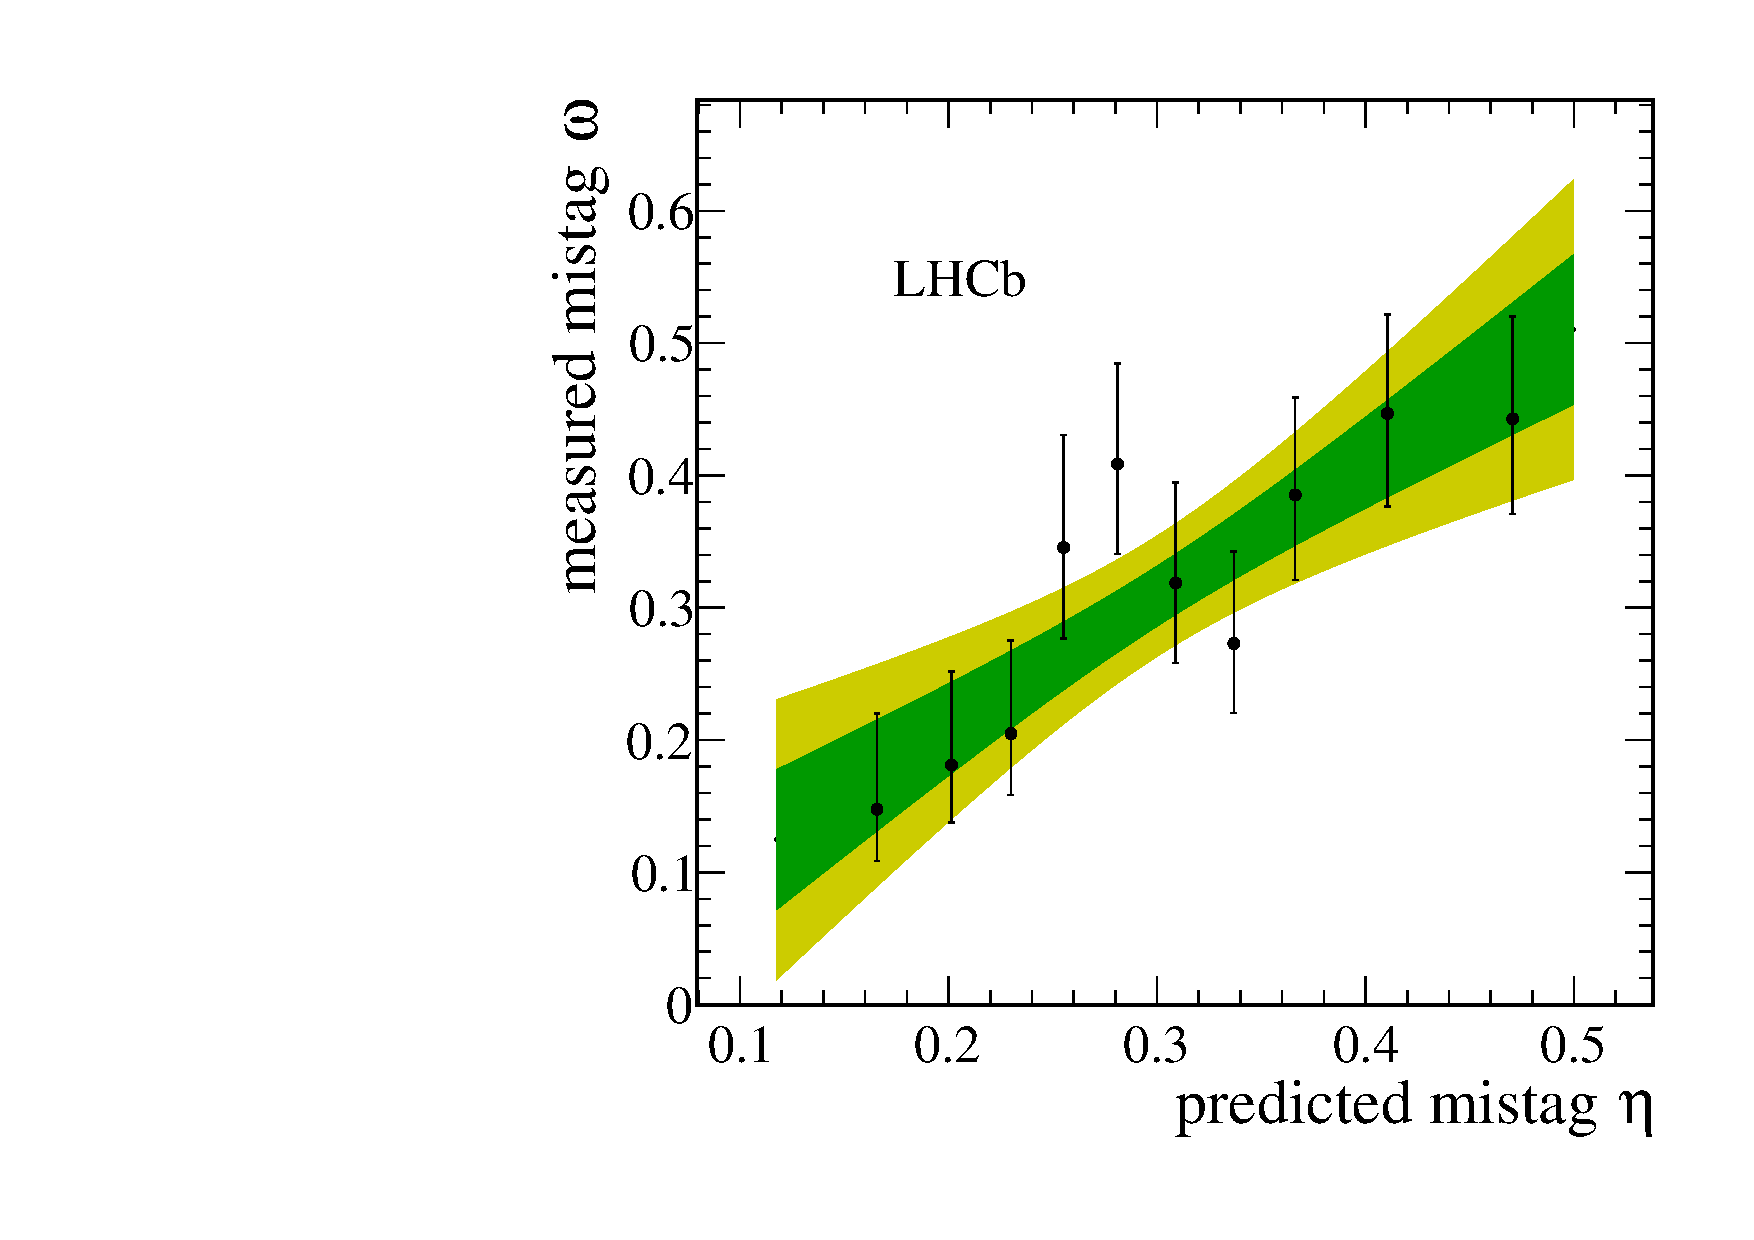
\includegraphics[height=!,width=0.33\textwidth]{figs/Tagging/Run1/OS_Muon_Calibration.pdf}
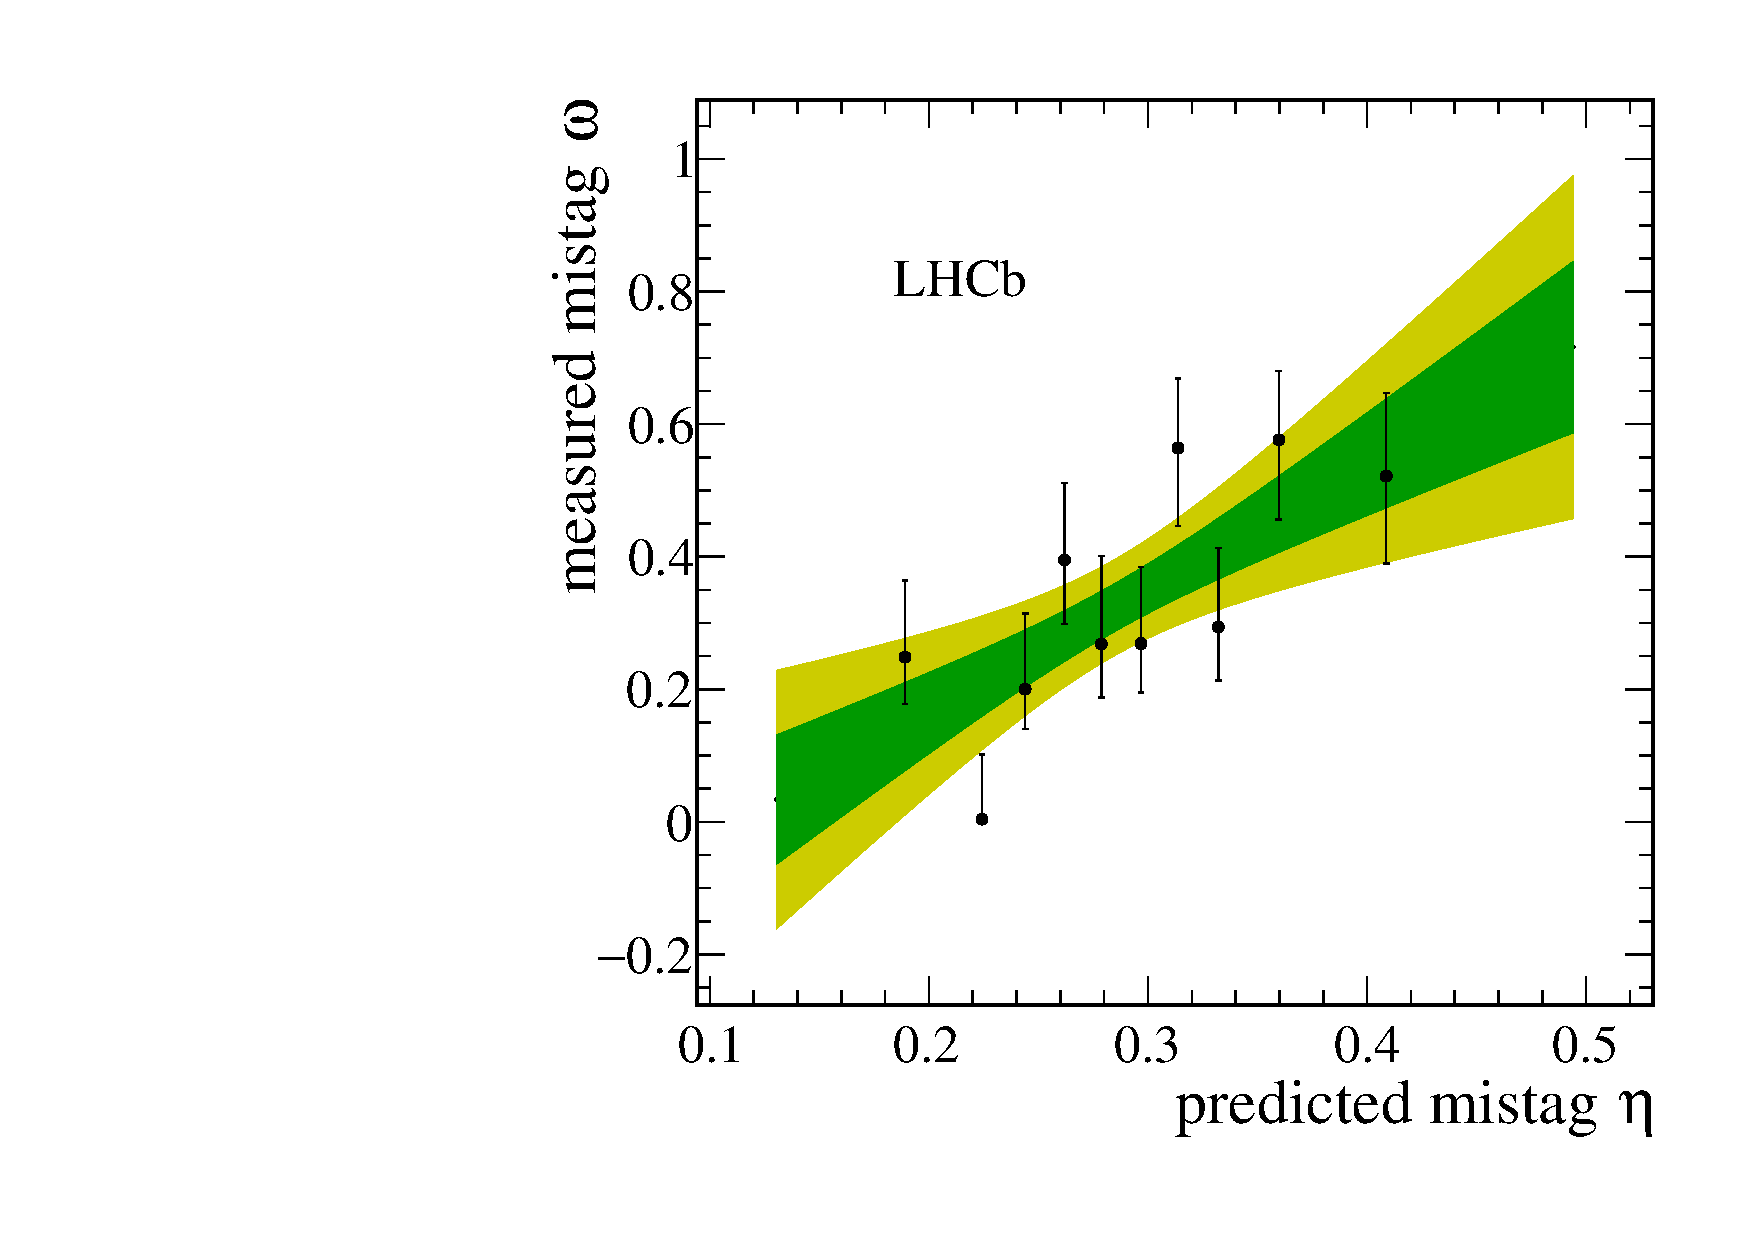
\includegraphics[height=!,width=0.33\textwidth]{figs/Tagging/Run1/OS_Electron_Calibration.pdf}

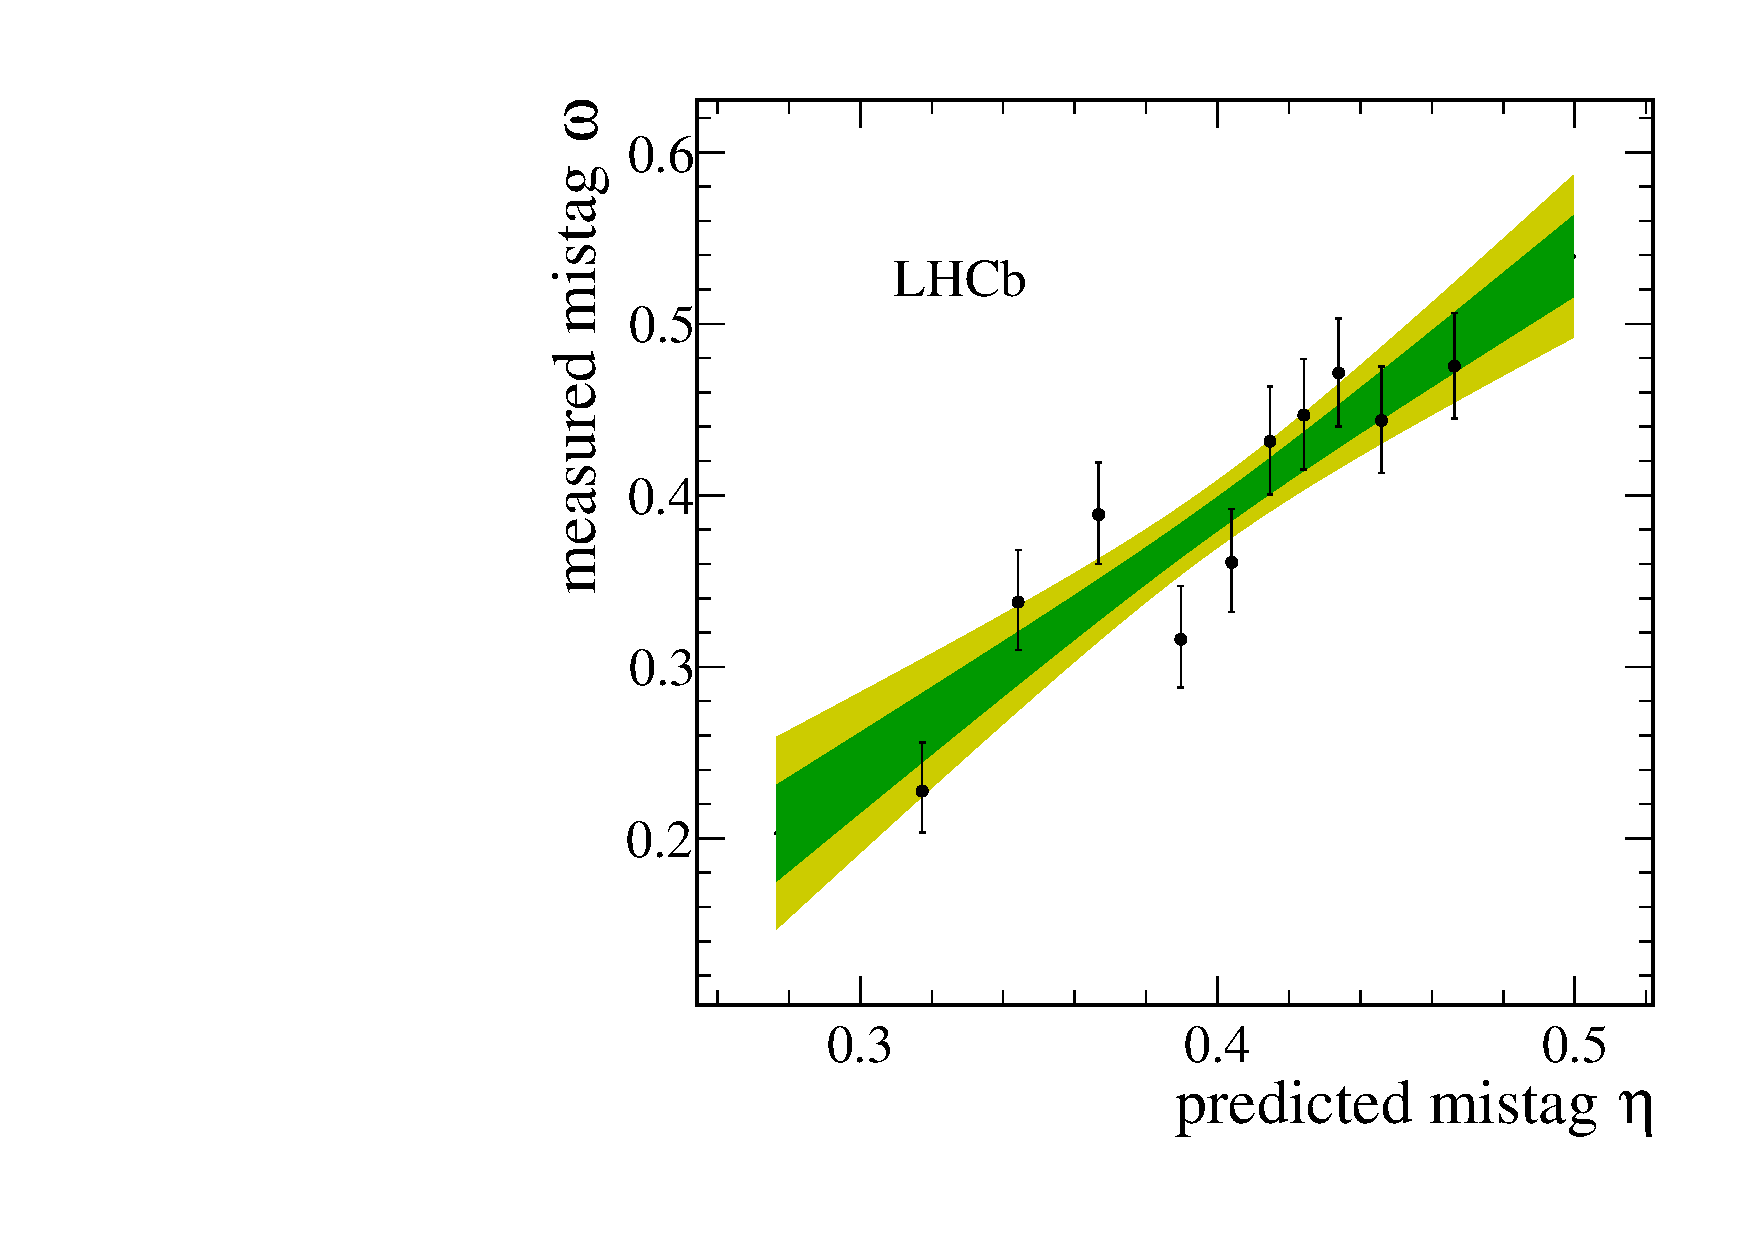
\includegraphics[height=!,width=0.33\textwidth]{figs/Tagging/Run1/OS_nnetKaon_Calibration.pdf}
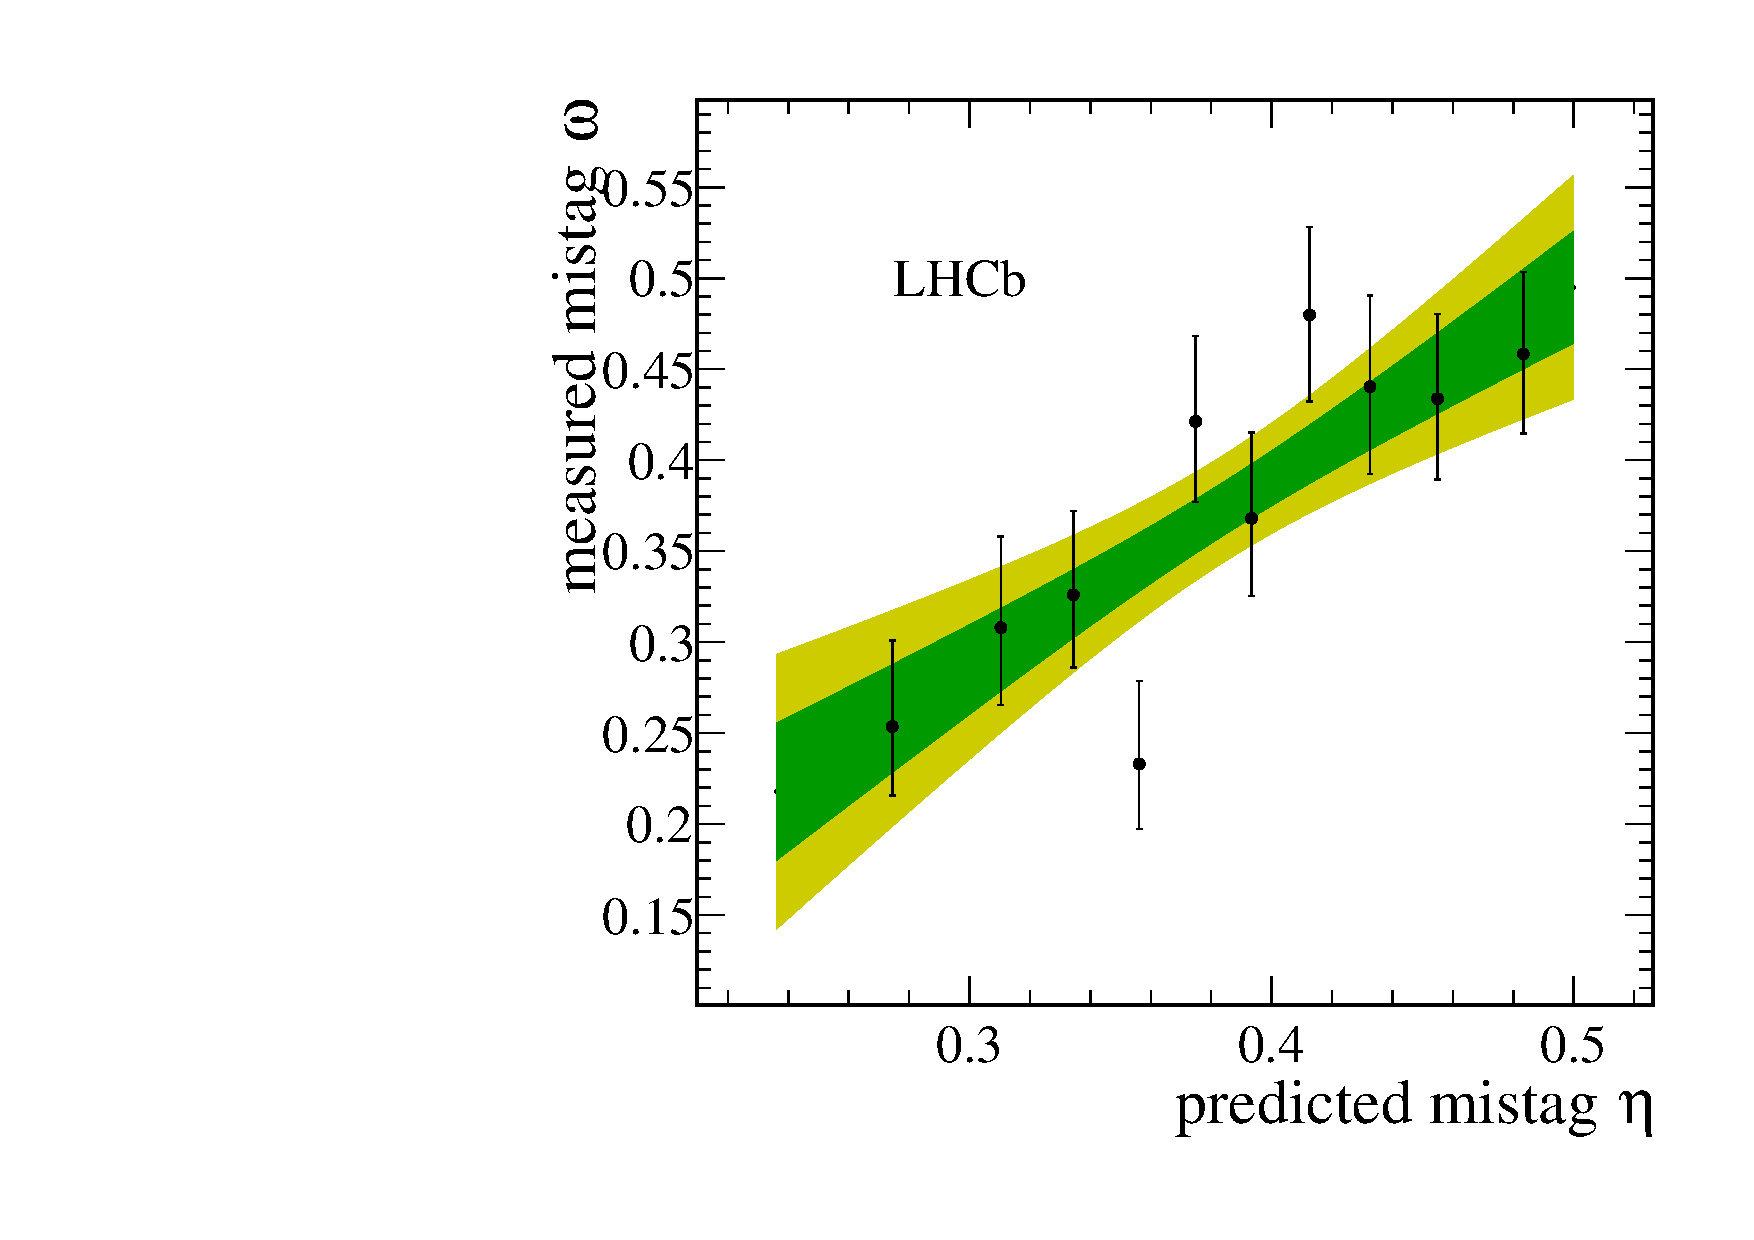
\includegraphics[height=!,width=0.33\textwidth]{figs/Tagging/Run1/VtxCharge_Calibration.pdf}
\caption{\small Predicted versus measured mistag probability for the (top left) OS muon, (top right) OS electron, (bottom left) OS kaon and (bottom right) OS vertex charge tagger for Run-I. 
A linear fit, including the $1\sigma$ and $2\sigma$ error bands is overlaid for each tagger.}
\label{fig:OSdistribution_Run1}
%\end{figure}
%
%\begin{figure}[h]
\centering
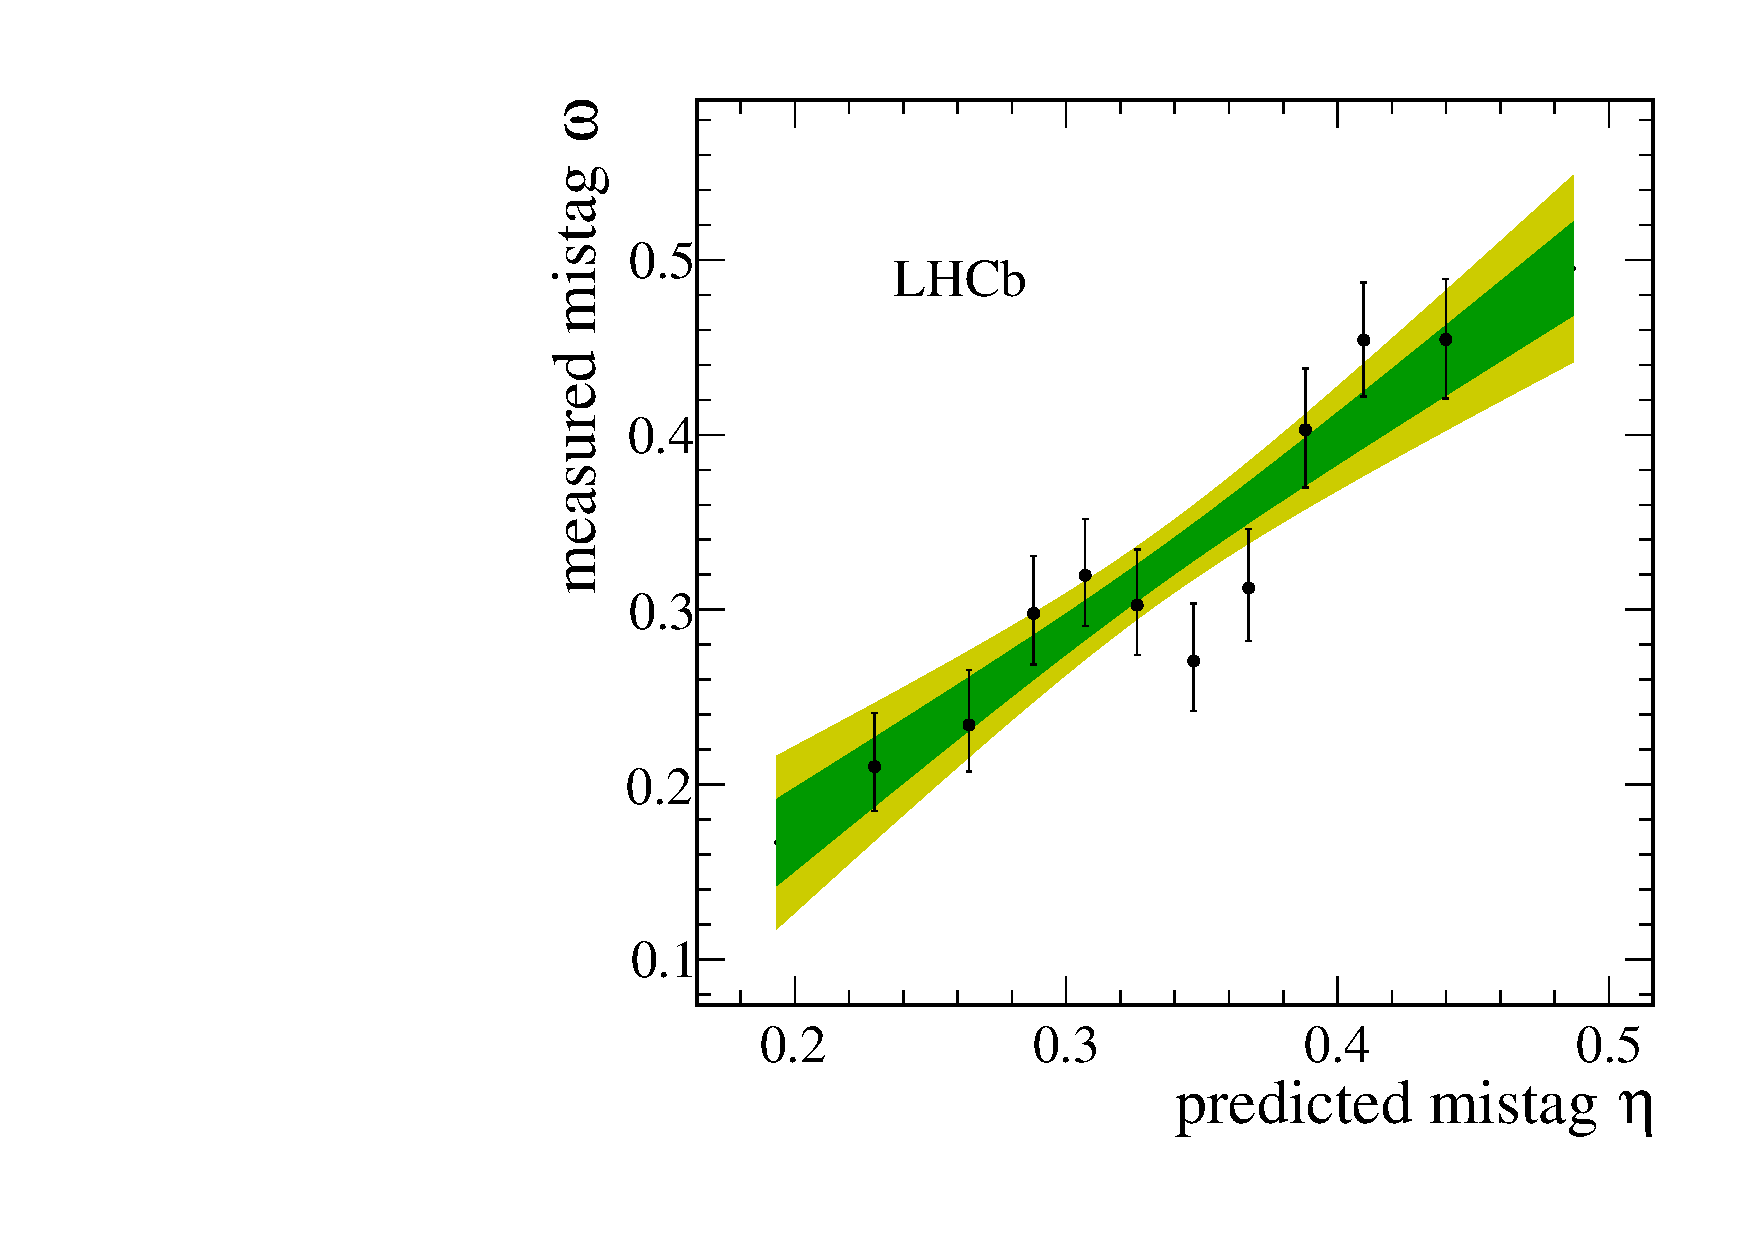
\includegraphics[height=!,width=0.33\textwidth]{figs/Tagging/Run2/OS_Muon_Calibration.pdf}
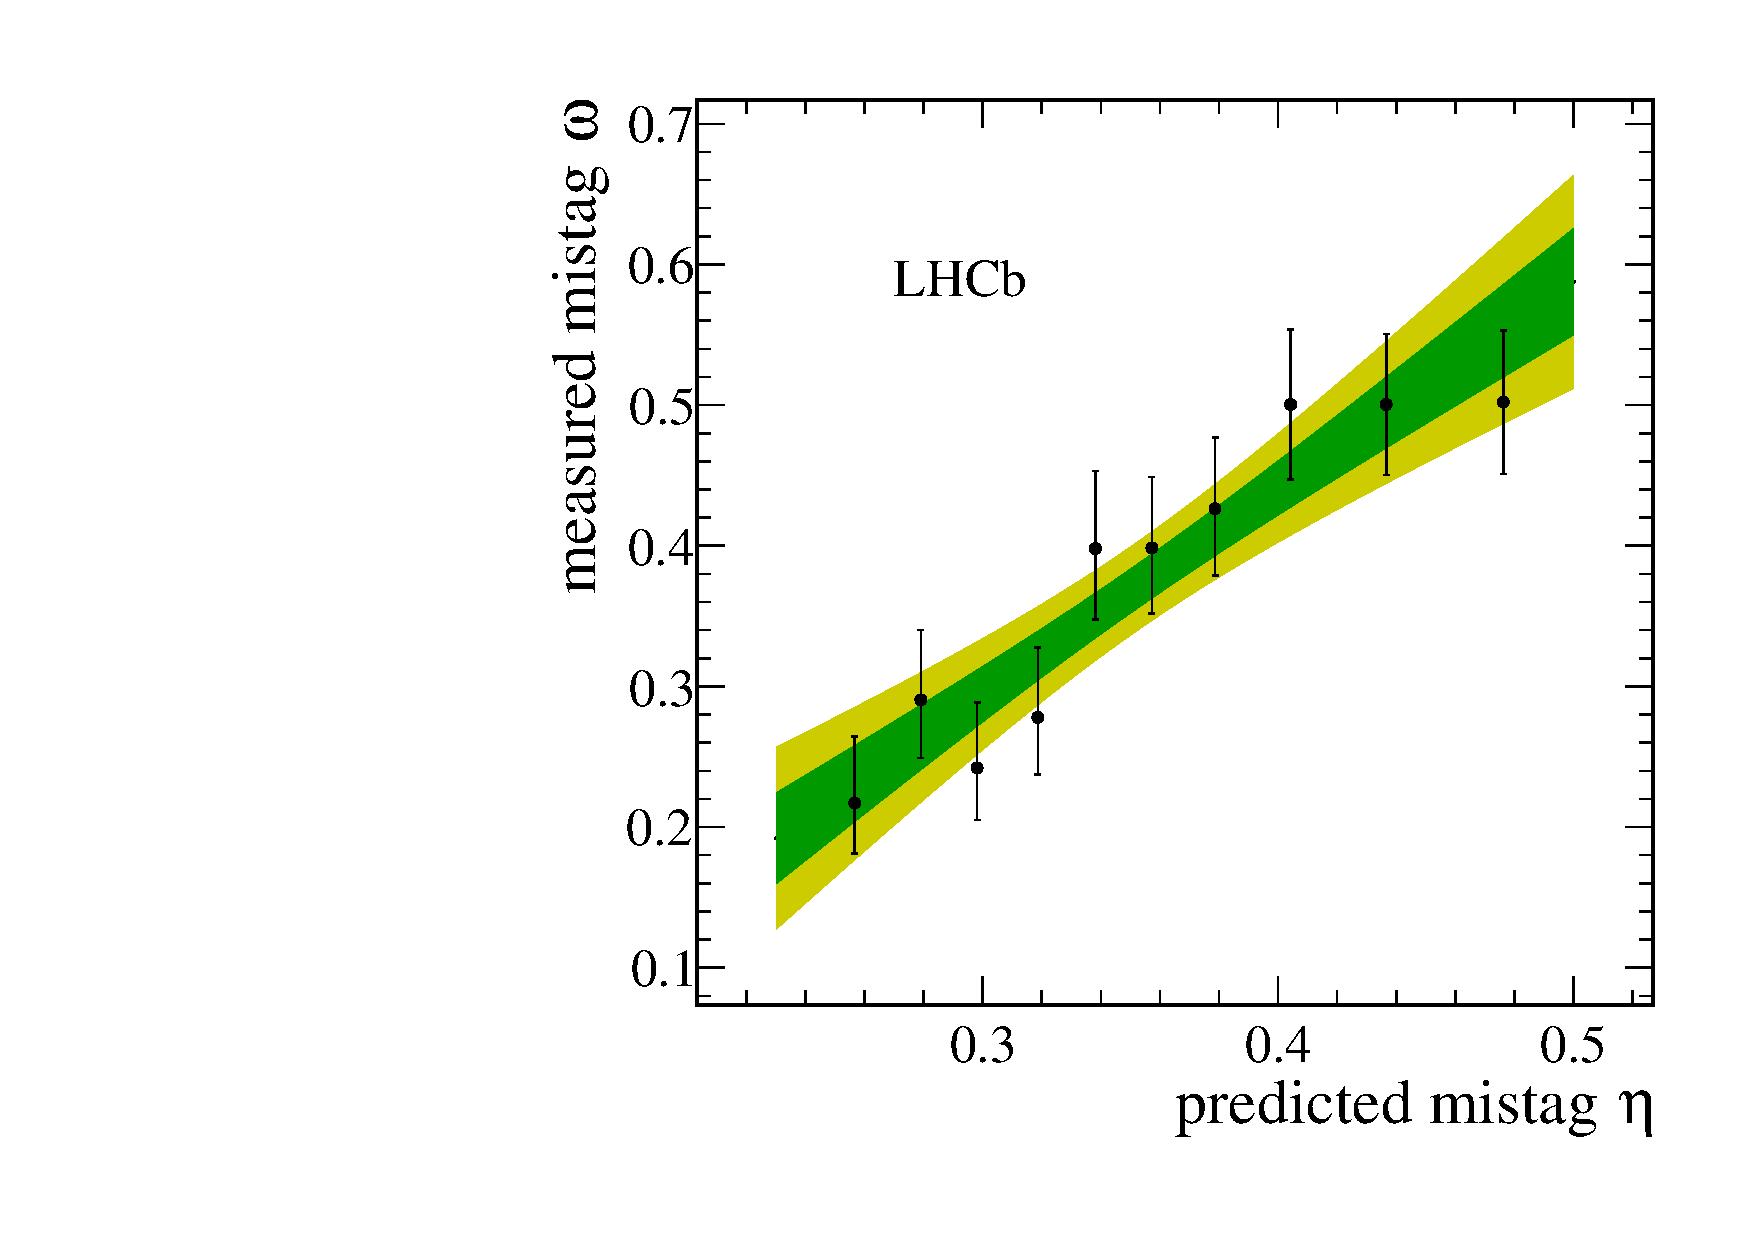
\includegraphics[height=!,width=0.33\textwidth]{figs/Tagging/Run2/OS_Electron_Calibration.pdf}

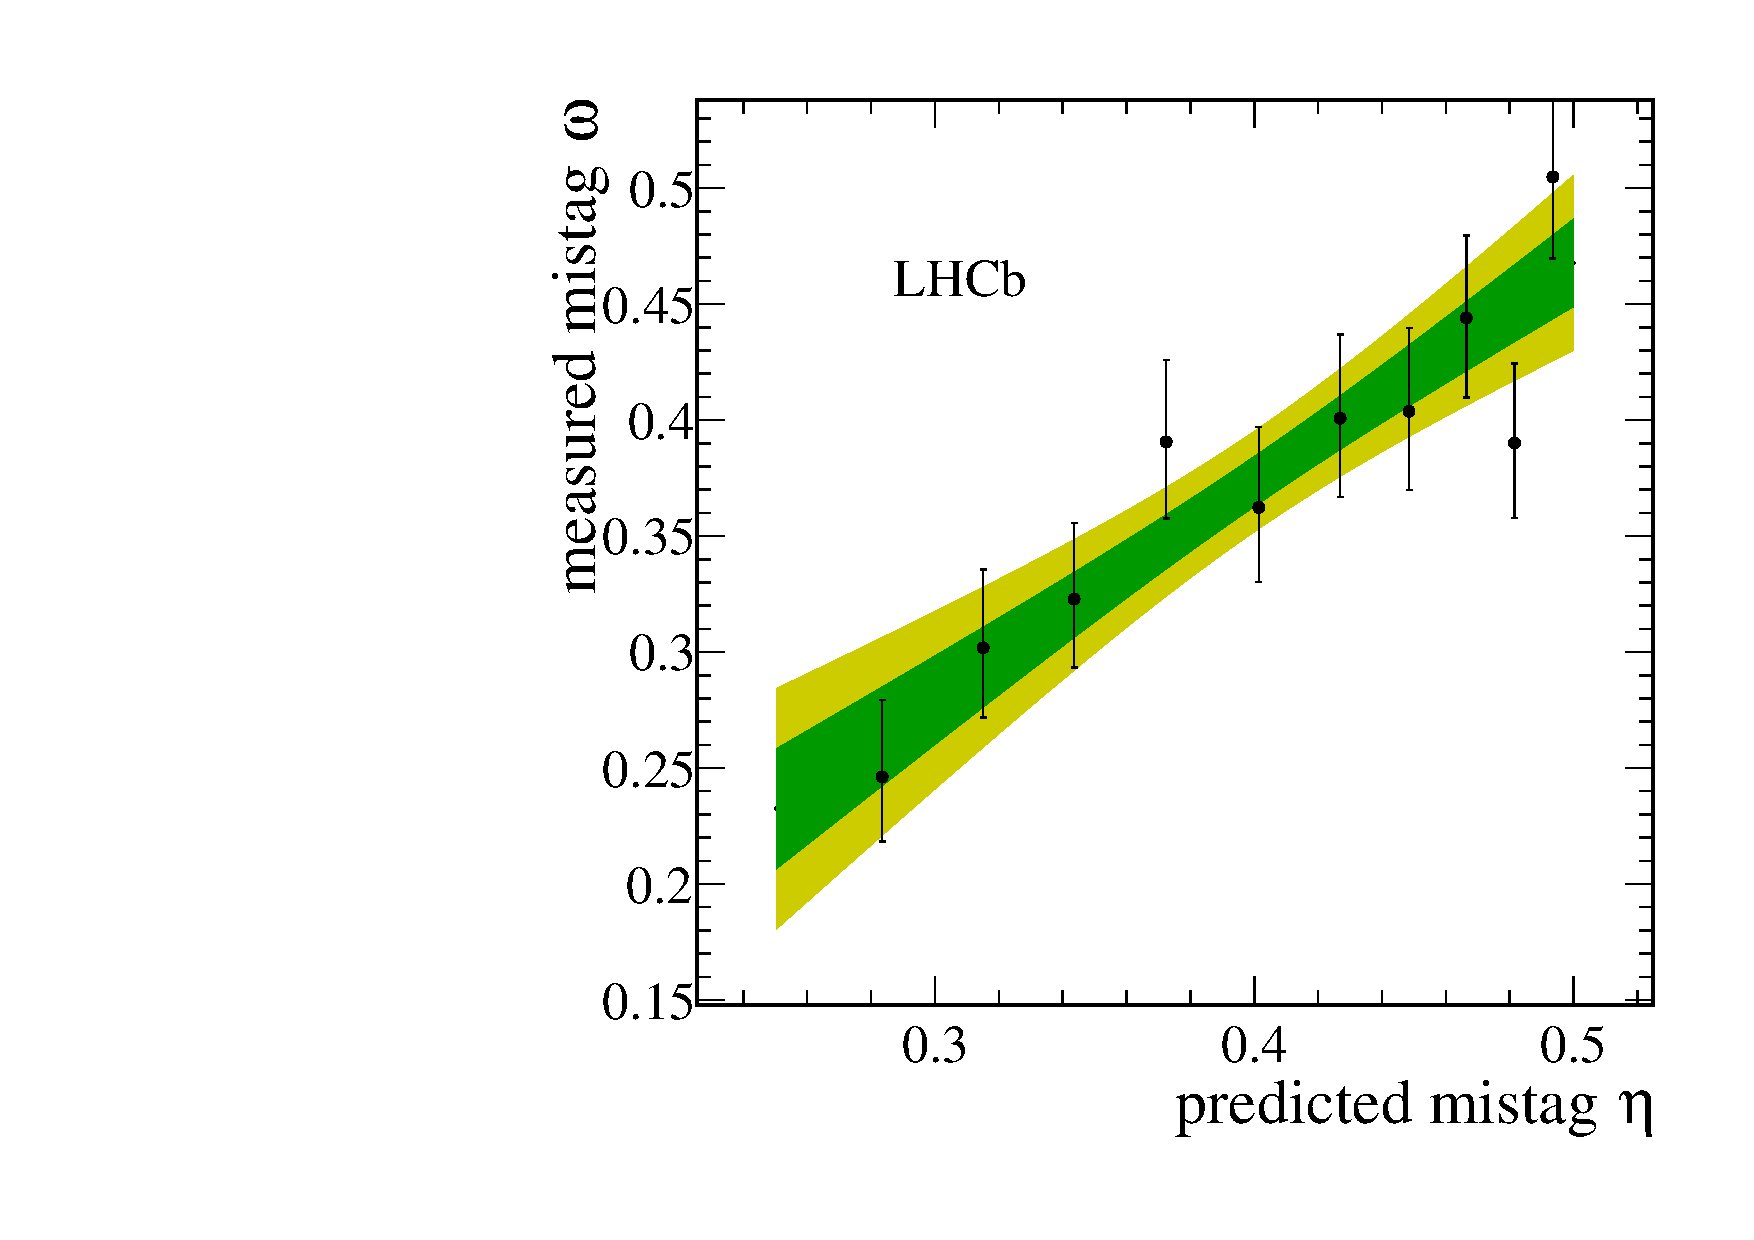
\includegraphics[height=!,width=0.33\textwidth]{figs/Tagging/Run2/OS_nnetKaon_Calibration.pdf}
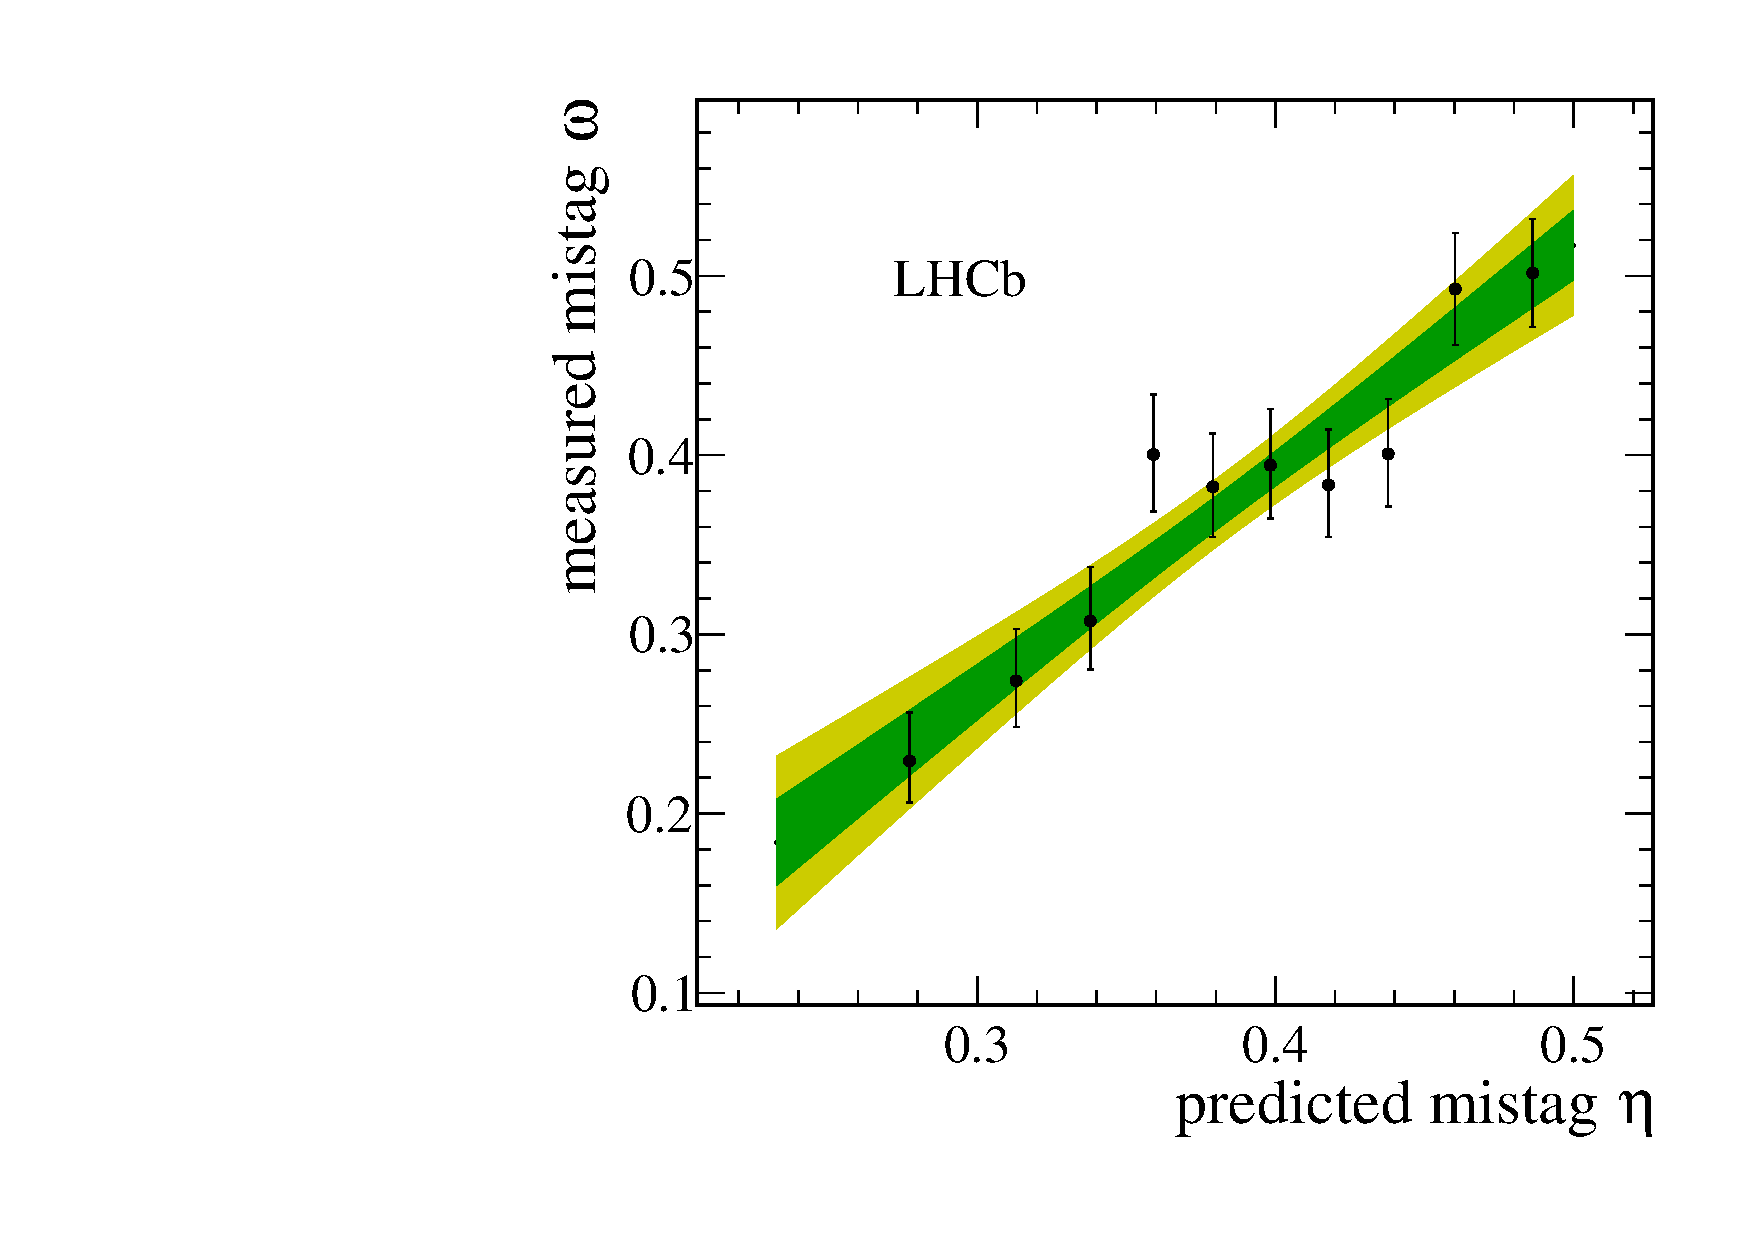
\includegraphics[height=!,width=0.33\textwidth]{figs/Tagging/Run2/VtxCharge_Calibration.pdf}
\caption{\small Predicted versus measured mistag probability for the (top left) OS muon, (top right) OS electron, (bottom left) OS kaon and (bottom right) OS vertex charge tagger for Run-II. 
A linear fit, including the $1\sigma$ and $2\sigma$ error bands is overlaid for each tagger.}
\label{fig:OSdistribution_Run2}
\end{figure}

\clearpage
\begin{table}[h]
\centering
%\scriptsize
\caption{The flavour tagging performances for the used OS taggers for Run-I data.}
\resizebox{\linewidth}{!}{
	\begin{table}
\centering
\begin{tabular}{rlllll}
\multicolumn{1}{c}{Tagger} & \multicolumn{1}{c}{$\epsilon$} & \multicolumn{1}{c}{$\omega$} & \multicolumn{1}{c}{$\epsilon \langle D^2 \rangle = \epsilon \left( 1 - 2 \omega \right)^2$} \\ 
OS $\mu$& $(8.775\pm0.207)\%$& $(28.935\pm0.180(\textrm{stat})\pm2.288(\textrm{cal}))\%$& $(1.558\pm0.045(\textrm{stat})\pm0.338(\textrm{cal}))\%$\\
OS $e$& $(3.191\pm0.129)\%$& $(28.778\pm0.366(\textrm{stat})\pm3.636(\textrm{cal}))\%$& $(0.575\pm0.031(\textrm{stat})\pm0.197(\textrm{cal}))\%$\\
OS $K$ NN& $(32.099\pm0.342)\%$& $(38.405\pm0.094(\textrm{stat})\pm1.152(\textrm{cal}))\%$& $(1.726\pm0.033(\textrm{stat})\pm0.343(\textrm{cal}))\%$\\
Vertex Charge& $(21.797\pm0.302)\%$& $(35.672\pm0.092(\textrm{stat})\pm1.480(\textrm{cal}))\%$& $(1.790\pm0.034(\textrm{stat})\pm0.370(\textrm{cal}))\%$\\
\end{tabular}
\end{table}

}
\label{tab:OS_Run1}
%\end{table}
%
%\begin{table}[h]
\caption{The flavour tagging performances for the used OS taggers for Run-II data.}
\resizebox{\linewidth}{!}{
	\begin{table}
\centering
\begin{tabular}{rlllll}
\multicolumn{1}{c}{Tagger} & \multicolumn{1}{c}{$\epsilon$} & \multicolumn{1}{c}{$\omega$} & \multicolumn{1}{c}{$\epsilon \langle D^2 \rangle = \epsilon \left( 1 - 2 \omega \right)^2$} \\ 
OS $\mu$& $(8.775\pm0.207)\%$& $(28.935\pm0.180(\textrm{stat})\pm2.288(\textrm{cal}))\%$& $(1.558\pm0.045(\textrm{stat})\pm0.338(\textrm{cal}))\%$\\
OS $e$& $(3.191\pm0.129)\%$& $(28.778\pm0.366(\textrm{stat})\pm3.636(\textrm{cal}))\%$& $(0.575\pm0.031(\textrm{stat})\pm0.197(\textrm{cal}))\%$\\
OS $K$ NN& $(32.099\pm0.342)\%$& $(38.405\pm0.094(\textrm{stat})\pm1.152(\textrm{cal}))\%$& $(1.726\pm0.033(\textrm{stat})\pm0.343(\textrm{cal}))\%$\\
Vertex Charge& $(21.797\pm0.302)\%$& $(35.672\pm0.092(\textrm{stat})\pm1.480(\textrm{cal}))\%$& $(1.790\pm0.034(\textrm{stat})\pm0.370(\textrm{cal}))\%$\\
\end{tabular}
\end{table}

}
\label{tab:OS_Run2}
\end{table}

%\begin{table}[h]
%\centering
%\scriptsize
% \begin{tabular}{l l l l | l l | l}
%\hline
%$p_{0}$ & $p_{1}$ & $<\eta>$ & $\epsilon_{tag}$ & $\Delta p_{o}$ & $\Delta p_{1}$ & $\epsilon_{eff}$ [$\%$] \\
%\hline
%0.025 $\pm$0.005  & 0.944 $\pm$ 0.048 & 0.347 & 0.517 $\pm$ 0.002 & 0.028 $\pm$ 0.005 & 0.037 $\pm$ 0.045 & 4.81 $\pm$ 0.04 (stat) $\pm$ 0.37 (cal) \\
%\hline
%\end{tabular}
%\caption{Calibration parameters and tagging asymmetries of the OS tagger extracted from $\Bs\to\Ds\pion\pion\pion$ decays.}
%\label{table: OScalibration}
%\normalsize
%\end{table}


%\subsection{SS tagging calibration}
%\label{subsec: SScalibration}
%The SS neural net kaon tagger can be calibrated using the flavour-specific $\Bs\to\Ds\pion\pion\pion$ decay. Its development, performance and calibration is described in detail in \cite{Aaij:2016psi}. 
%Figure \ref{fig:SSdistribution} shows the distribution of the predicted mistag of the neural net kaon tagger. 
%The extracted calibration parameters and tagging asymmetries are summarized in Table \ref{table: SScalibration} and the measured tagging power for this algorithm is $\epsilon_{eff,SS} = 3.22  \%$.
%
%
%\begin{figure}[h]
%\centering
%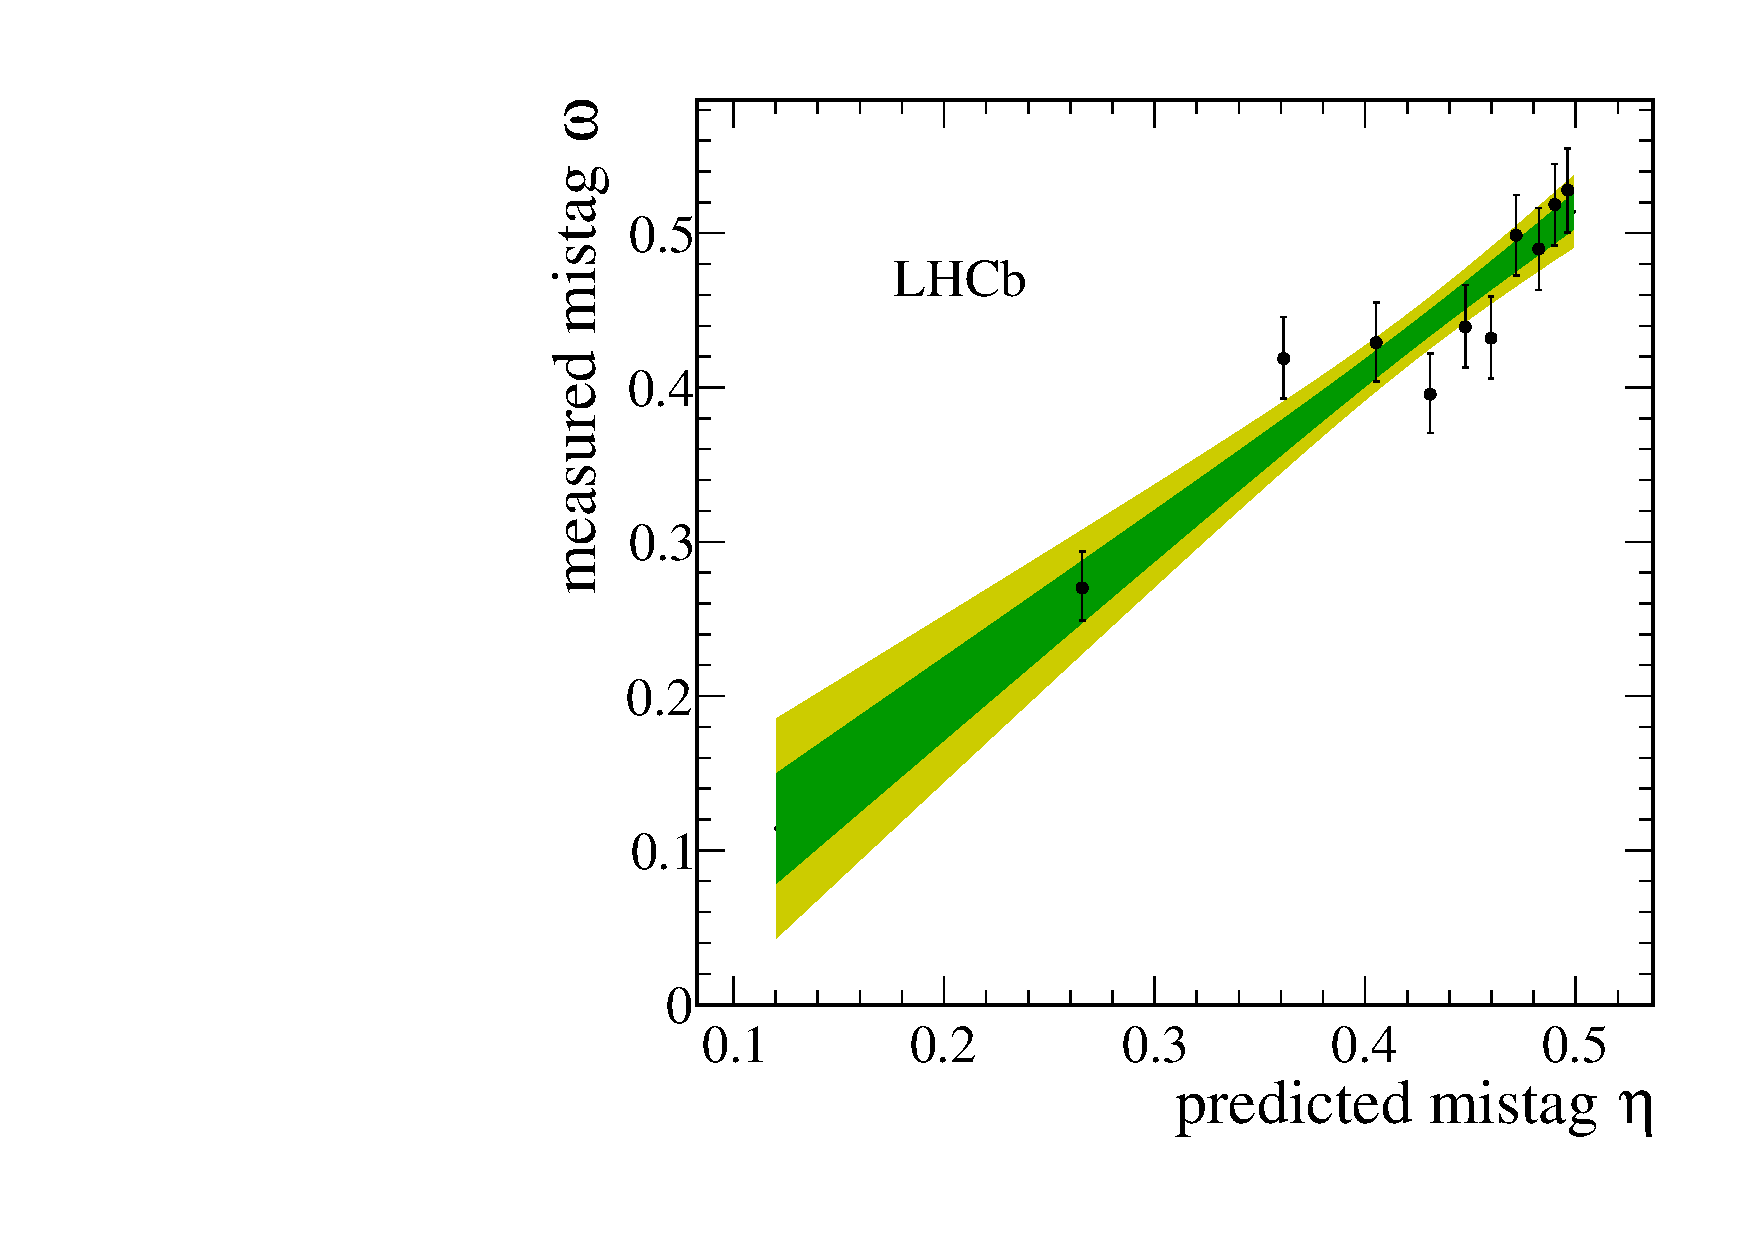
\includegraphics[height=!,width=0.4\textwidth]{figs/Tagging/Run1/SS_nnetKaon_Calibration.pdf}
%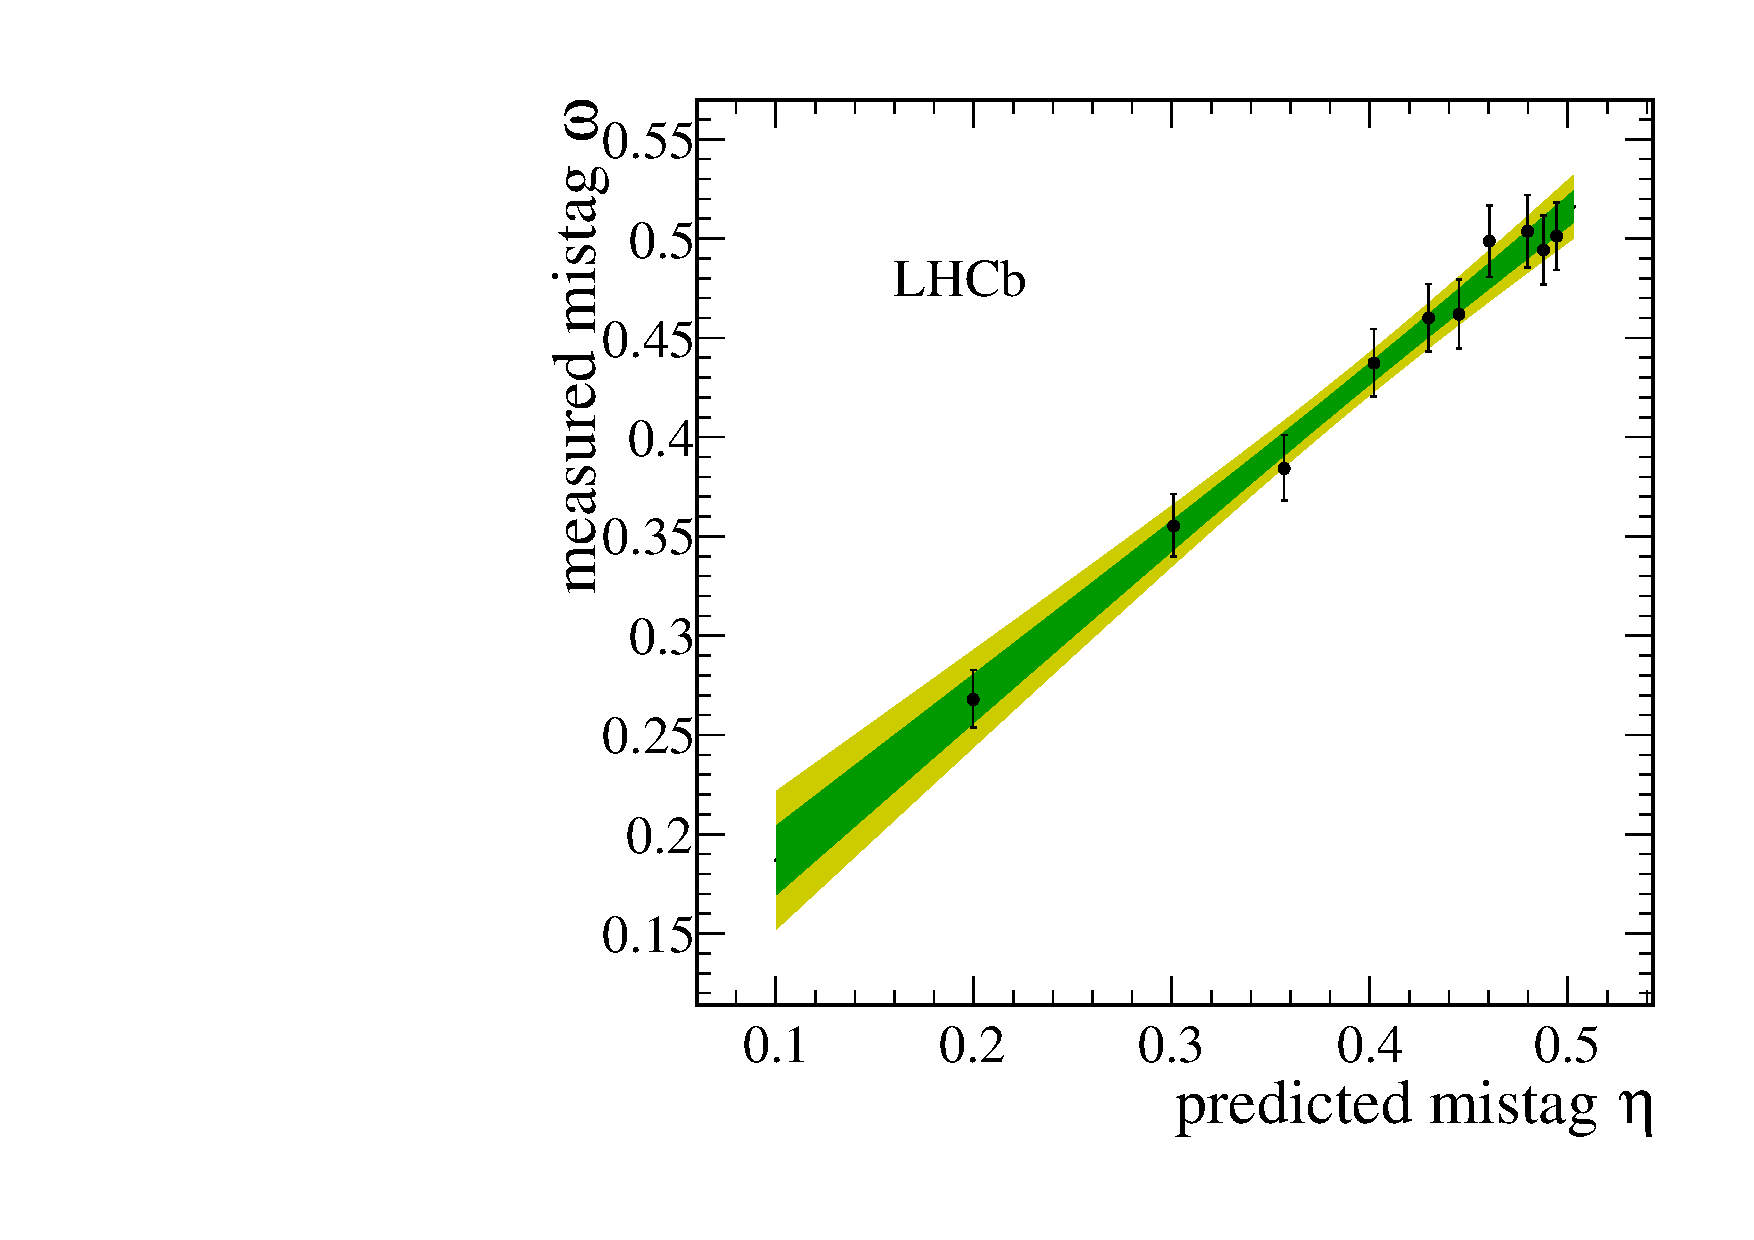
\includegraphics[height=!,width=0.4\textwidth]{figs/Tagging/Run2/SS_nnetKaon_Calibration.pdf}
%\caption{Predicted versus measured mistag probability for the SS neural net kaon tagger for (left) Run 1 and (right) Run 2. 
%A linear fit, including the $1\sigma$ and $2\sigma$ error bands is overlaid for both distributions.}
%\label{fig:SSdistribution}
%\end{figure}
%
%
%\begin{table}[h]
%\centering
%\scriptsize
% \begin{tabular}{l l l l | l l | l}
%\hline
%$p_{0}$ & $p_{1}$ & $<\eta>$ & $\epsilon_{tag}$ & $\Delta p_{o}$ & $\Delta p_{1}$ & $\epsilon_{eff}$ [$\%$] \\
%\hline
%0.008 $\pm$ 0.004  & 1.086 $\pm$ 0.059 & 0.381 & 0.571 $\pm$ 0.002 & -0.017 $\pm$ 0.004  & 0.135 $\pm$ 0.058 & 3.22 $\pm$ 0.03 (stat) $\pm$ 0.26 (cal) \\
%\hline
%\end{tabular}
%\caption{Calibration parameters and tagging asymmetries of the SS tagger extracted from $\Bs\to\Ds\pion\pion\pion$ decays.}
%\label{table: SScalibration}
%\normalsize
%\end{table}

\subsection{Tagging performance}
\label{subsec:TaggingComparison}

The OS-Combo and SS-Kaon taggers are calibrated simultaneously by fitting the $B_s \to D_s \pi\pi\pi$ decay-time distribution as discussed in Sec.~\ref{sec:timeFit}.
The predicted mistag probabilities $\eta_{OS}$ and $\eta_{SS}$, shown Fig.~\ref{fig:w_data_comparison} for $B_s \to D_s \pi\pi\pi$ and $B_s \to D_s K\pi\pi$ data,
are included as per-event observables, effectively giving a larger weight to the events that have a lower mistag probability.
The tagger responses are combined into a single response on an event-by-event basis during the fit.
Tables \ref{tab:tagPerfRun1} and \ref{tab:tagPerfRun2} report the tagging performances for the OS and SS combination 
considering three mutually exclusive categories of tagged events: OS only, SS only and both OS and SS.


%To justify the usage of the tagging calibration, obtained using the $\Bs\to\Ds\pion\pion\pion$ sample, for our signal decay, the performance of the taggers in the two decay channels needs to be compatible. 
%This is verified using both, simulated signal samples of both decays and sweighted data, 
%to compare the similarity of the mistag probabilities, tagging decisions and kinematic observables that are correlated with the tagging response, on simulation and data.  \newline
% 
%\begin{figure}[h]
%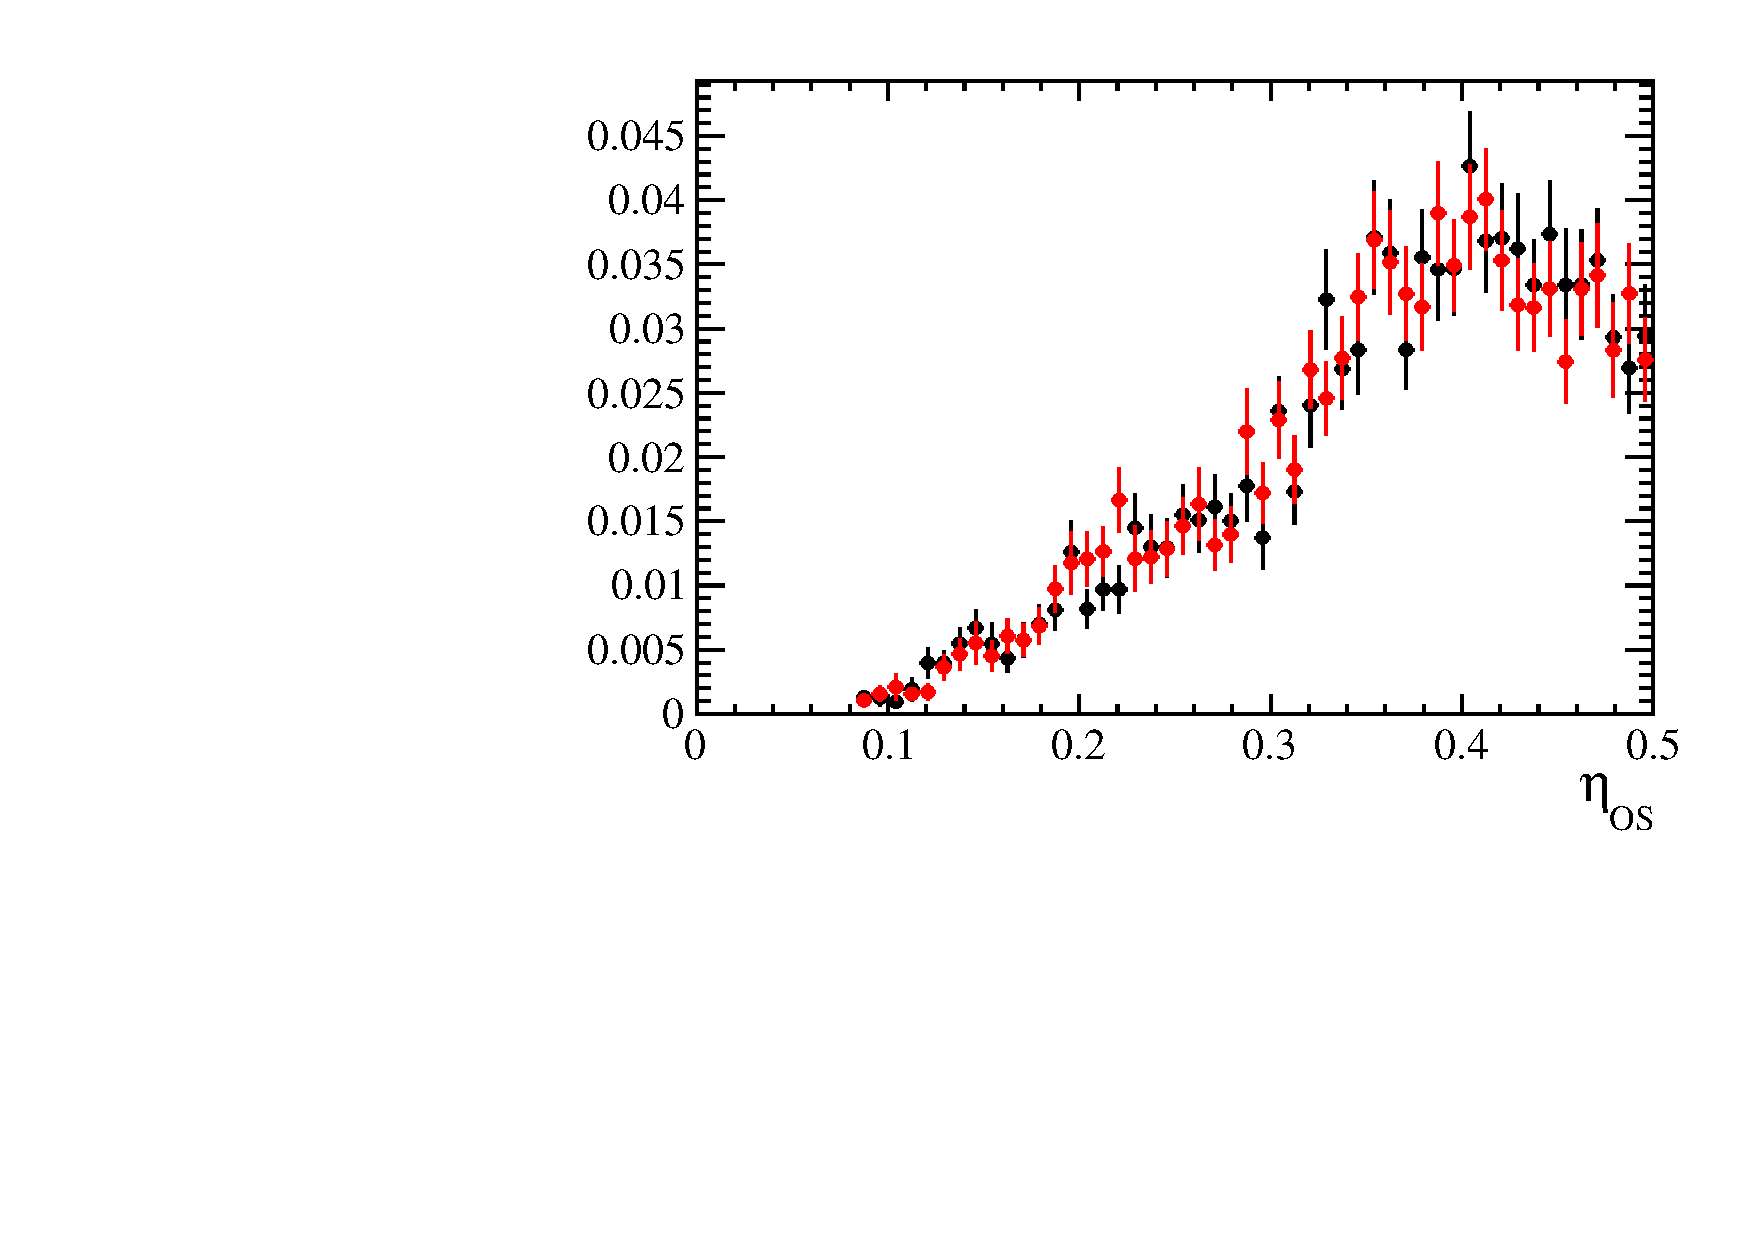
\includegraphics[height=7.cm,width=0.49\textwidth]{figs/Tagging/w_OS_MC.pdf}
%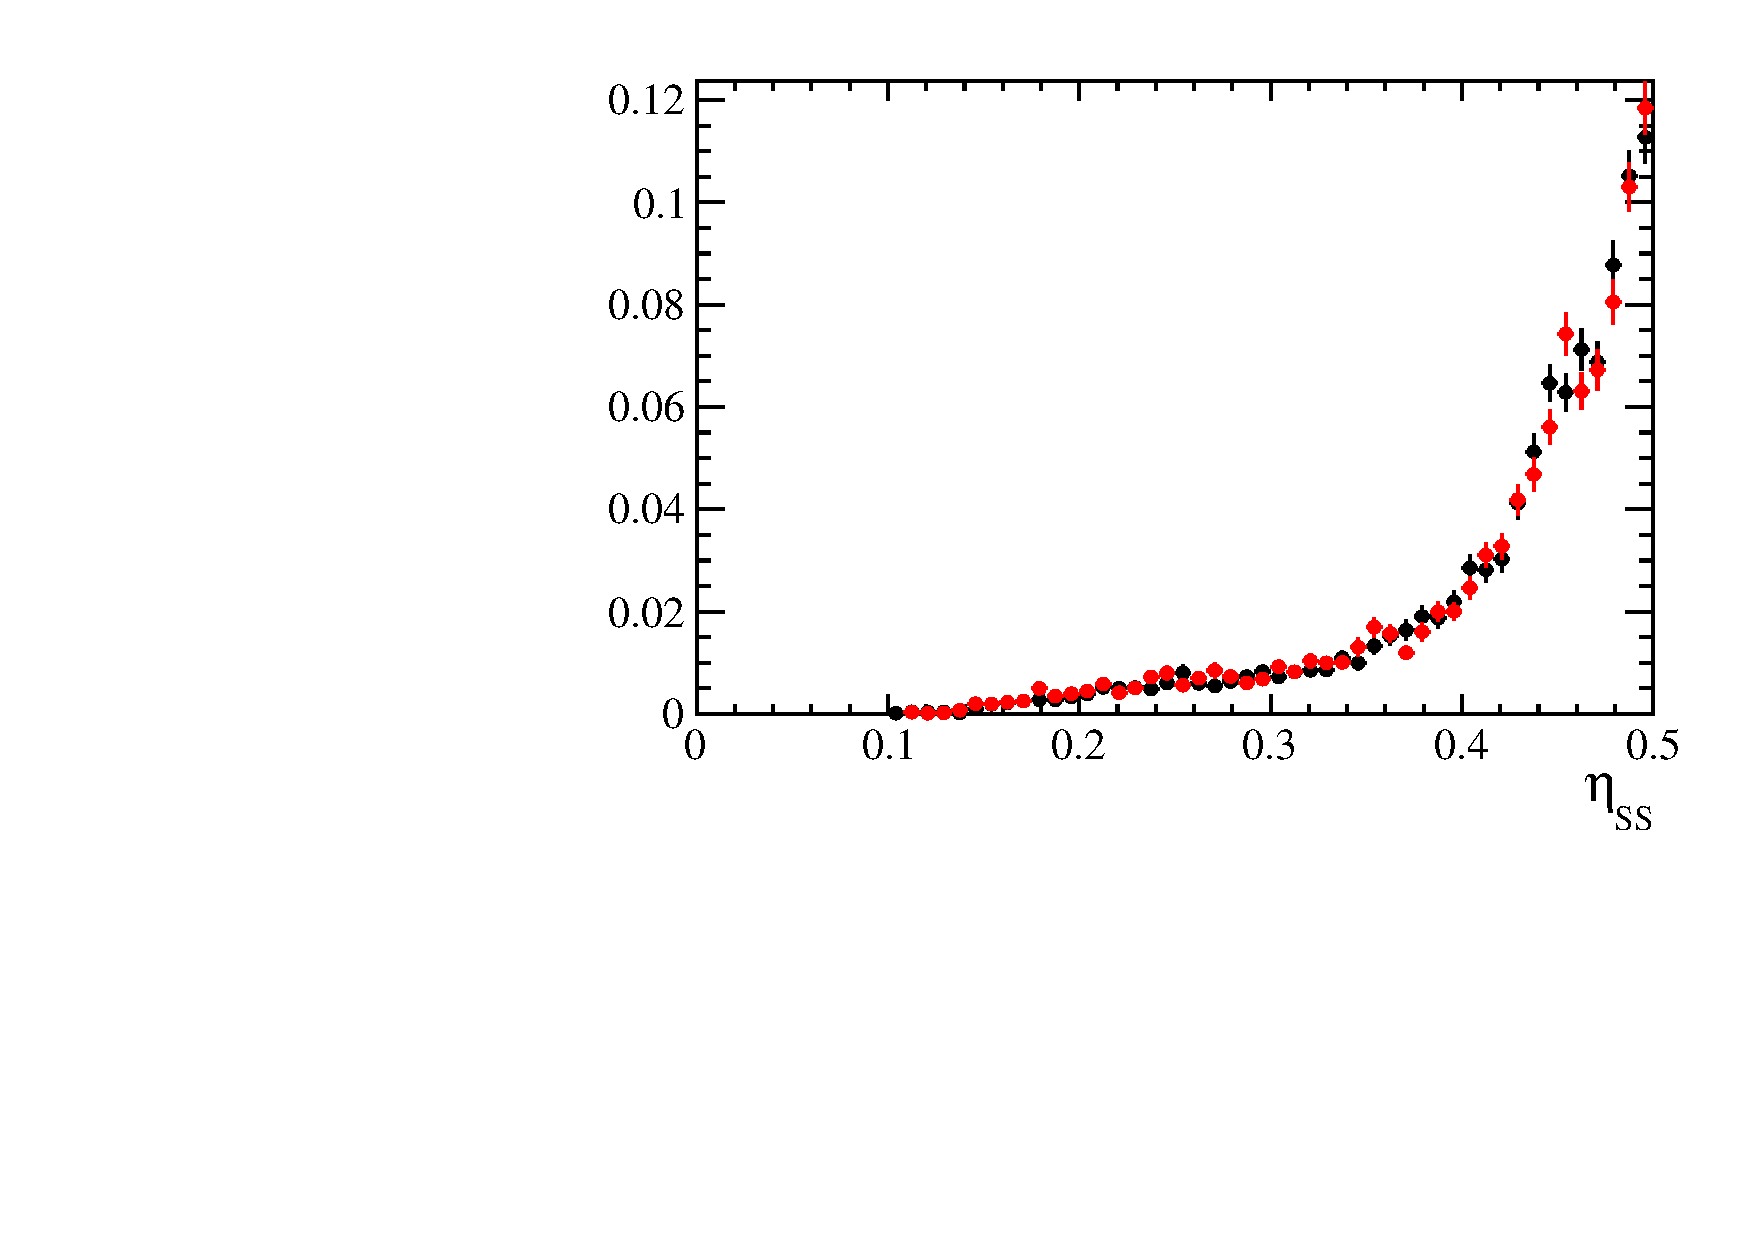
\includegraphics[height=7.cm,width=0.49\textwidth]{figs/Tagging/w_SS_MC.pdf}
%\caption{Distributions of the predicted mistag $\eta$ for the OS combination (left) and the SS kaon tagger (right) in simulated $\Bs\to\Ds\kaon\pion\pion$ (black) and $\Bs\to\Ds\pion\pion\pion$ (red) signal.}
%\label{fig:w_MC_comparison}
%\end{figure}

\begin{figure}[h]
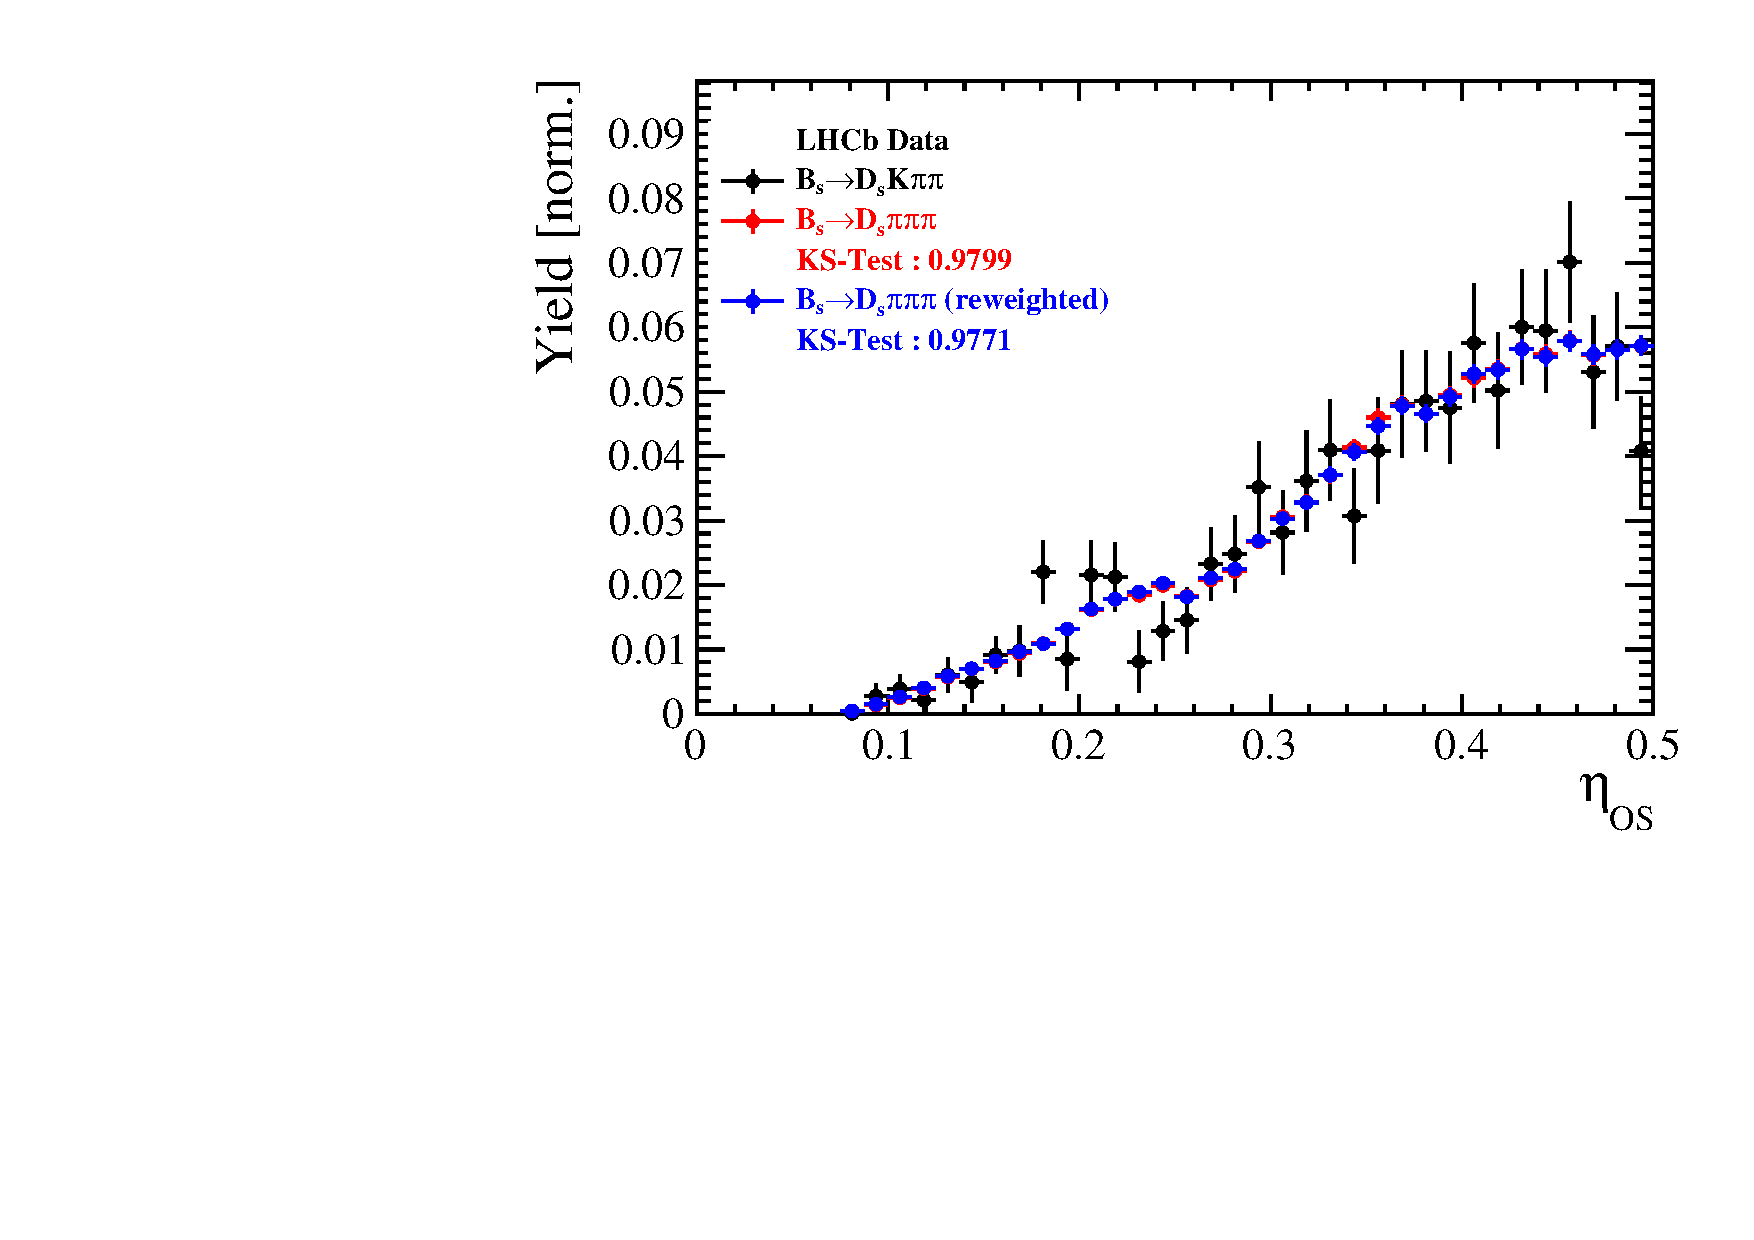
\includegraphics[height=!,width=0.5\textwidth]{figs/dataVsMC/norm2signal/Ds2all_Bs_TAGOMEGA_OS.pdf}
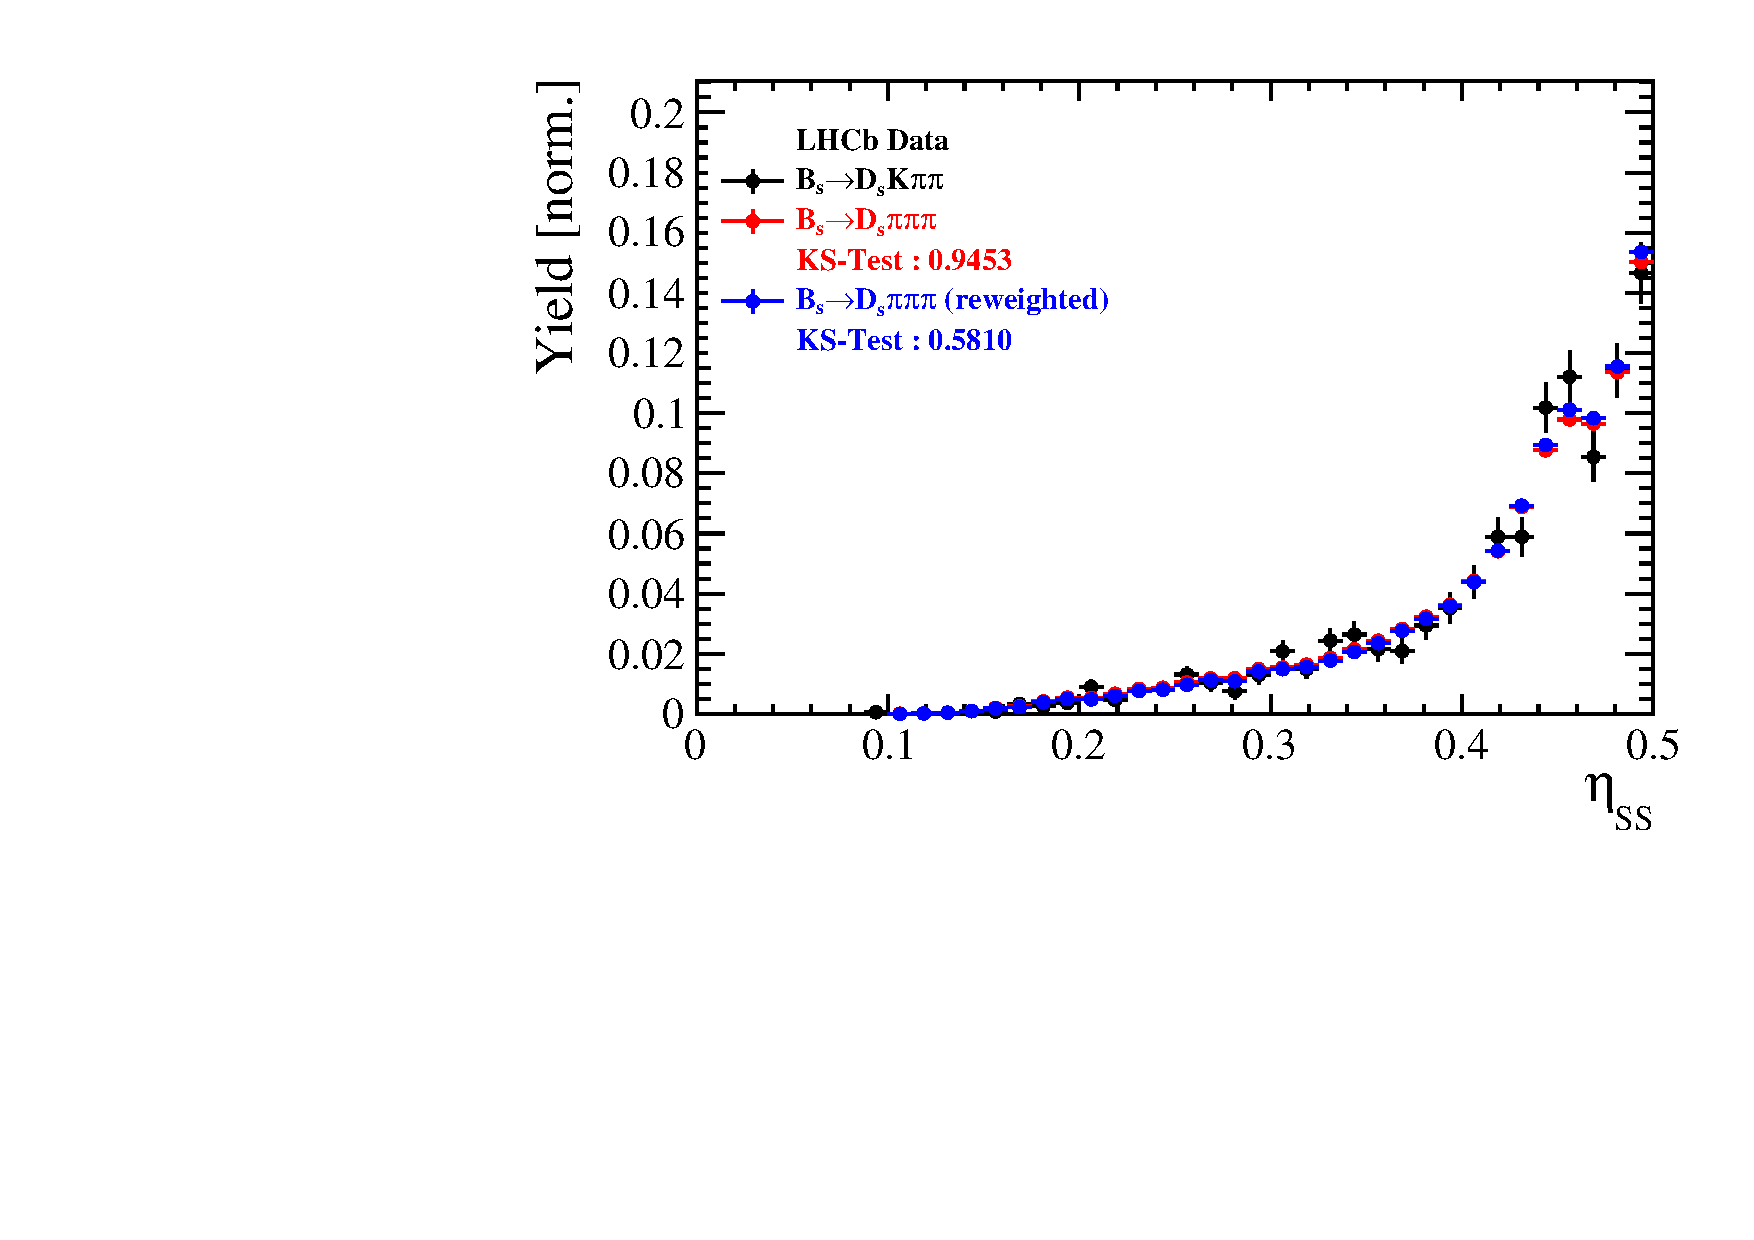
\includegraphics[height=!,width=0.5\textwidth]{figs/dataVsMC/norm2signal/Ds2all_Bs_SS_nnetKaon_PROB.pdf}
\caption{Distributions of the predicted mistag $\eta$ for the OS combination (left) and the SS kaon tagger (right) 
for signal candidates in the $\Bs\to\Ds\kaon\pion\pion$ (black) and $\Bs\to\Ds\pion\pion\pion$ (red) data samples.}
\label{fig:w_data_comparison}
\end{figure}
%Both, data and simulated samples, show good agreement between the signal and normalization channel. 
%Compatibility is also seen in Fig. \ref{fig:tagDec_data_comparison}, which shows the comparison of the tagging decision distributions of the OS and SS tagger for sweighted data. 

%\begin{figure}[h]
%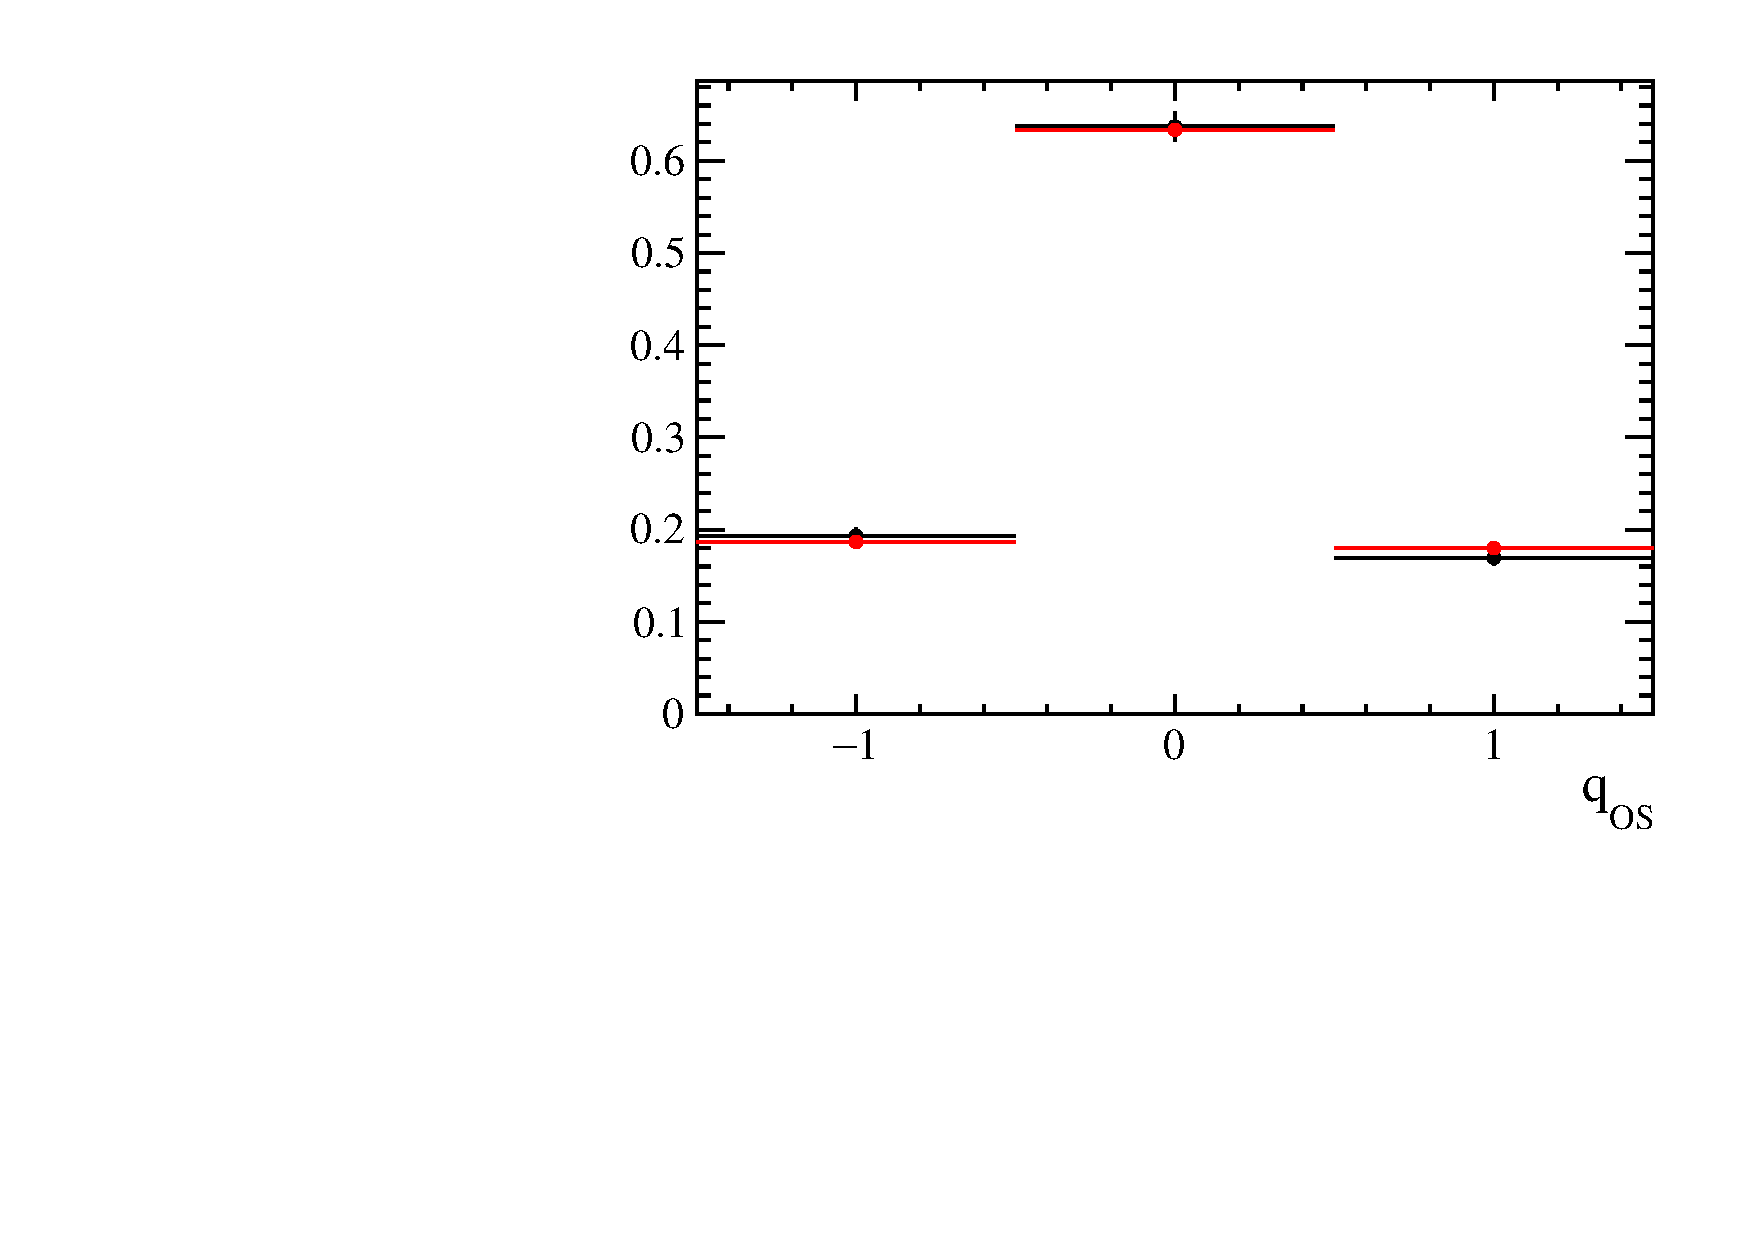
\includegraphics[height=7.cm,width=0.49\textwidth]{figs/Tagging/qOS.pdf}
%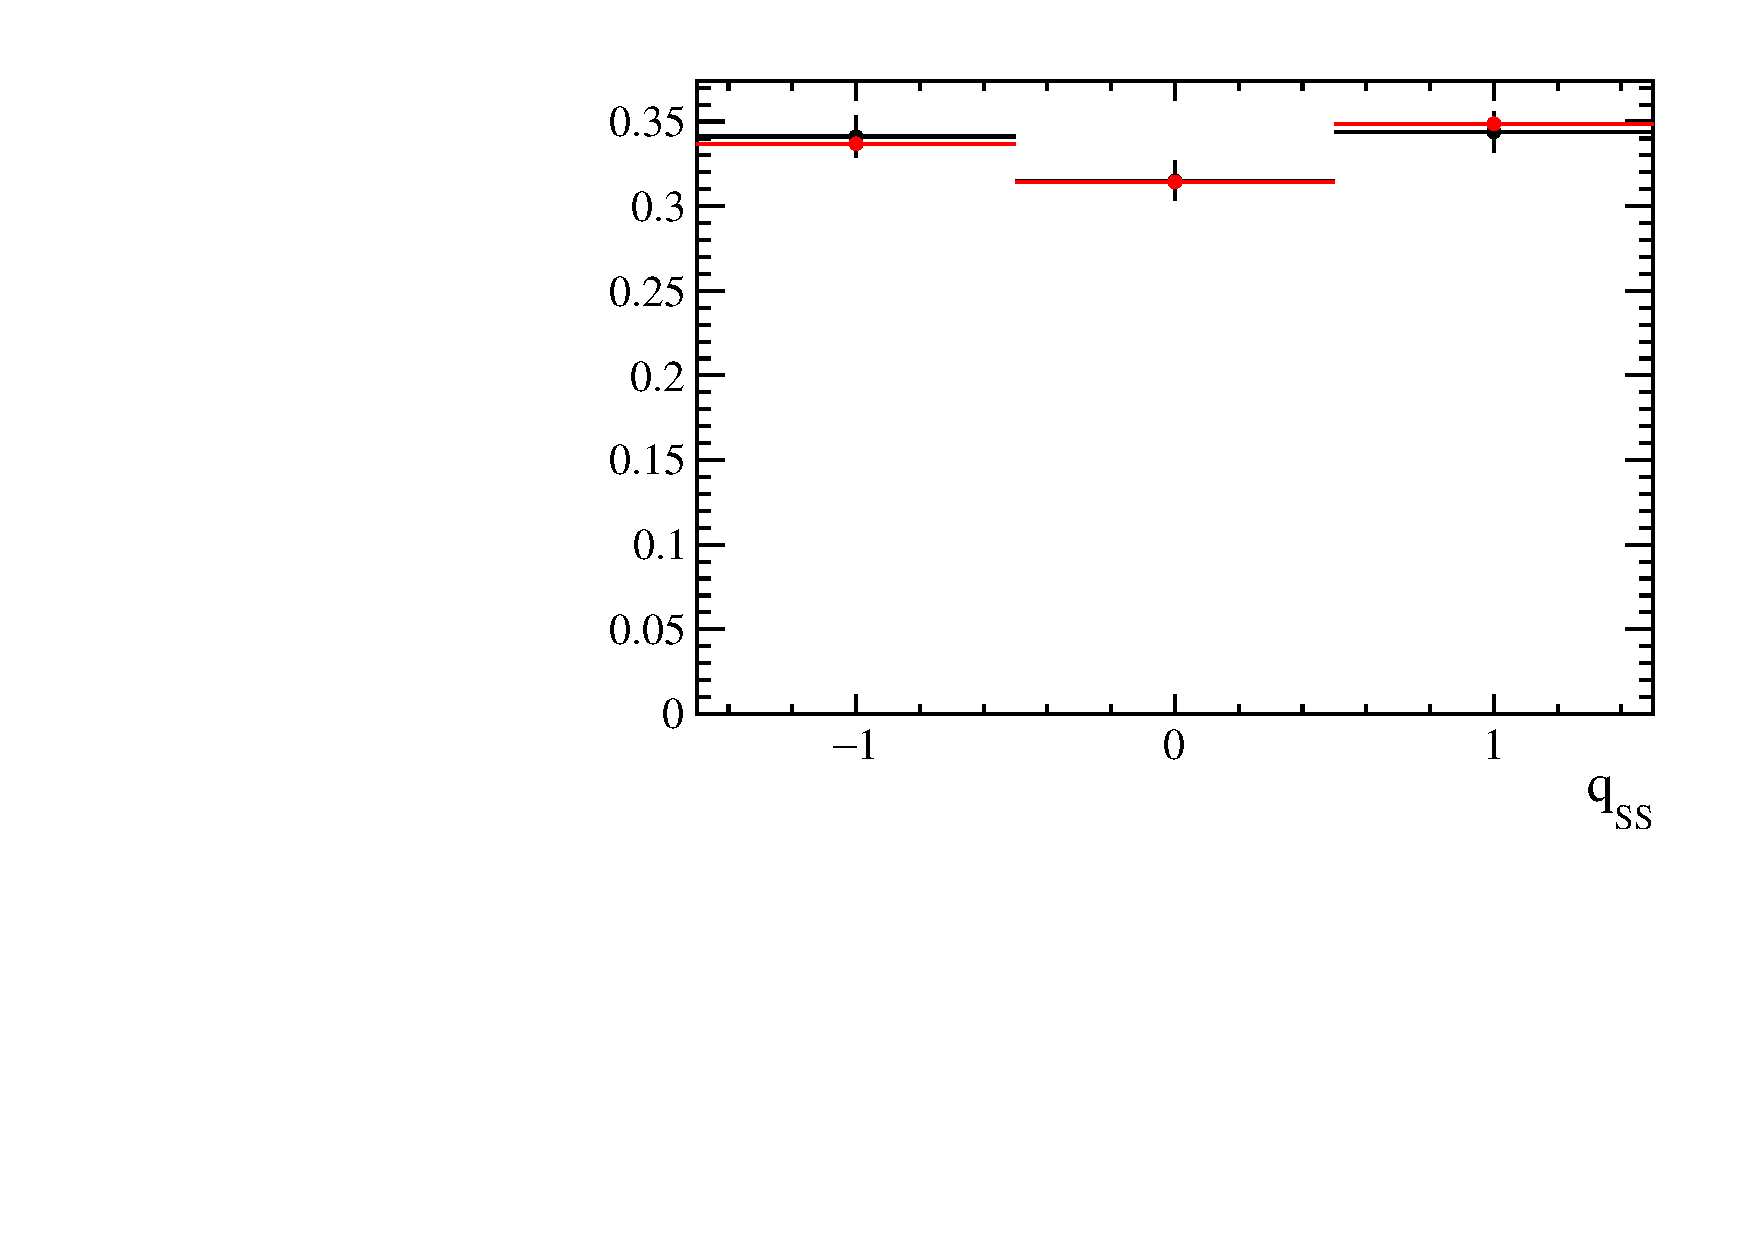
\includegraphics[height=7.cm,width=0.49\textwidth]{figs/Tagging/q_SS.pdf}
%\caption{Distributions of the tagging decision from the OS combination (left) and the SS kaon tagger (right) for signal candidates in the $\Bs\to\Ds\kaon\pion\pion$ (black) and $\Bs\to\Ds\pion\pion\pion$ (red) data samples. 
%The signal distributions are obtained using sWeights, the procedure is described in Sec. \ref{subsec: sWegihts}.}
%\label{fig:tagDec_data_comparison}
%\end{figure}


%\begin{figure}[h]
%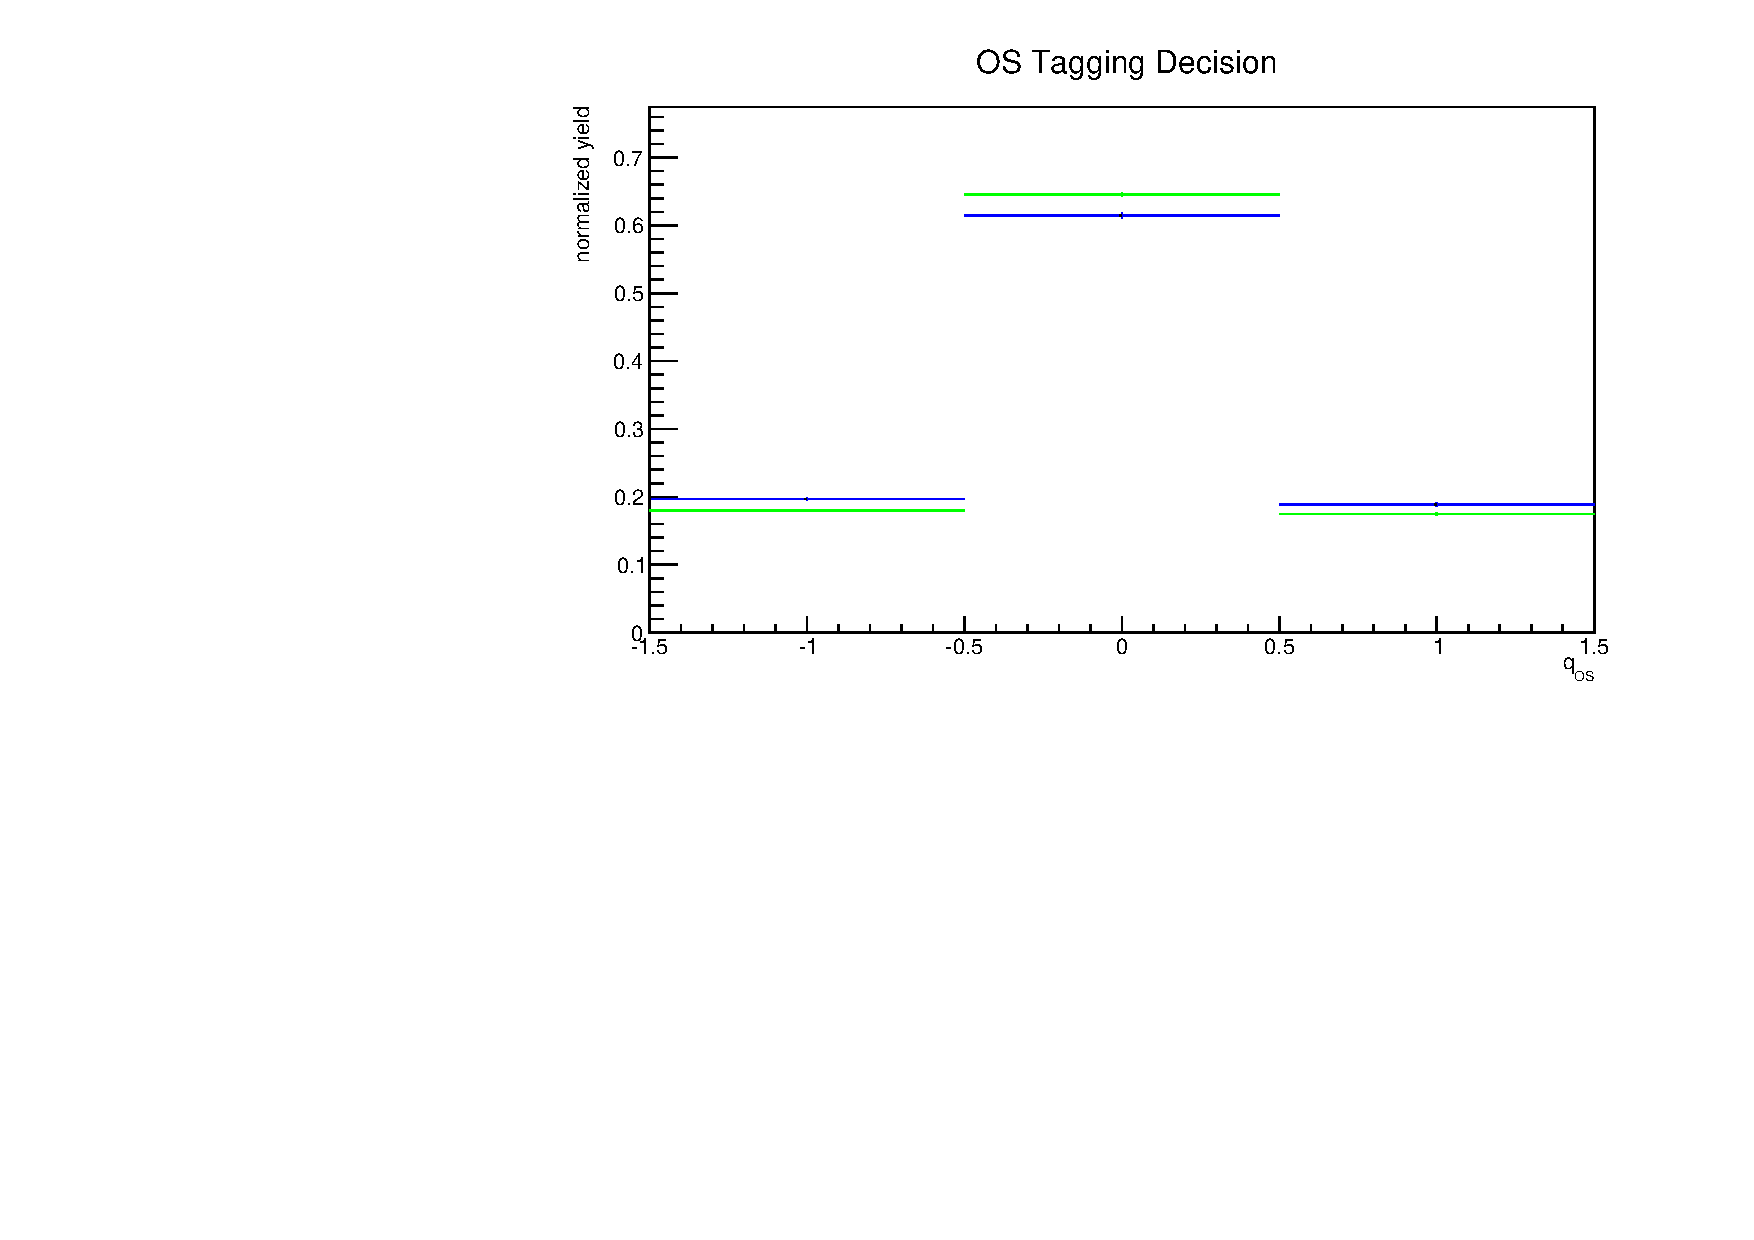
\includegraphics[height=7.cm,width=0.49\textwidth]{figs/Tagging/OS_Combination_DEC_norm_RunsComparison.pdf}
%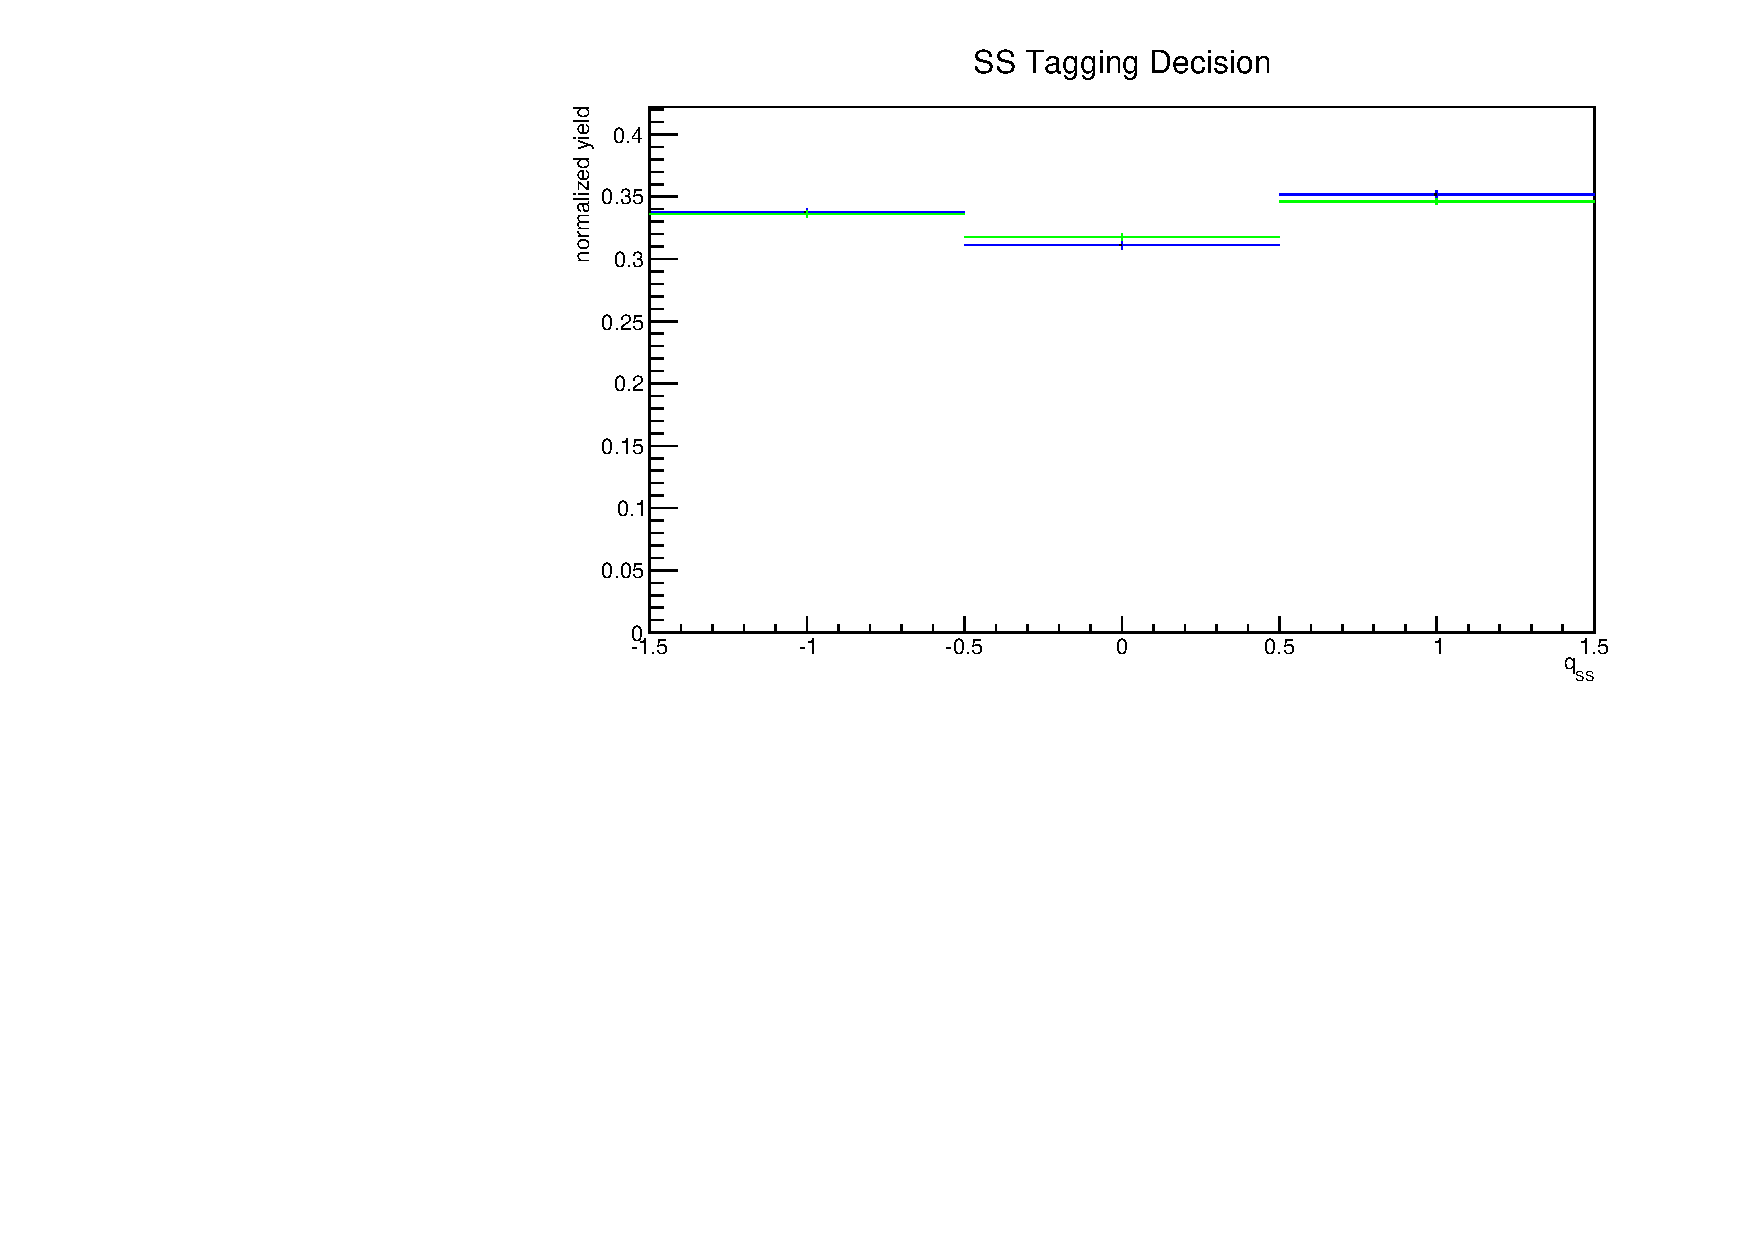
\includegraphics[height=7.cm,width=0.49\textwidth]{figs/Tagging/SS_nnetKaon_DEC_norm_RunsComparison.pdf}\\
%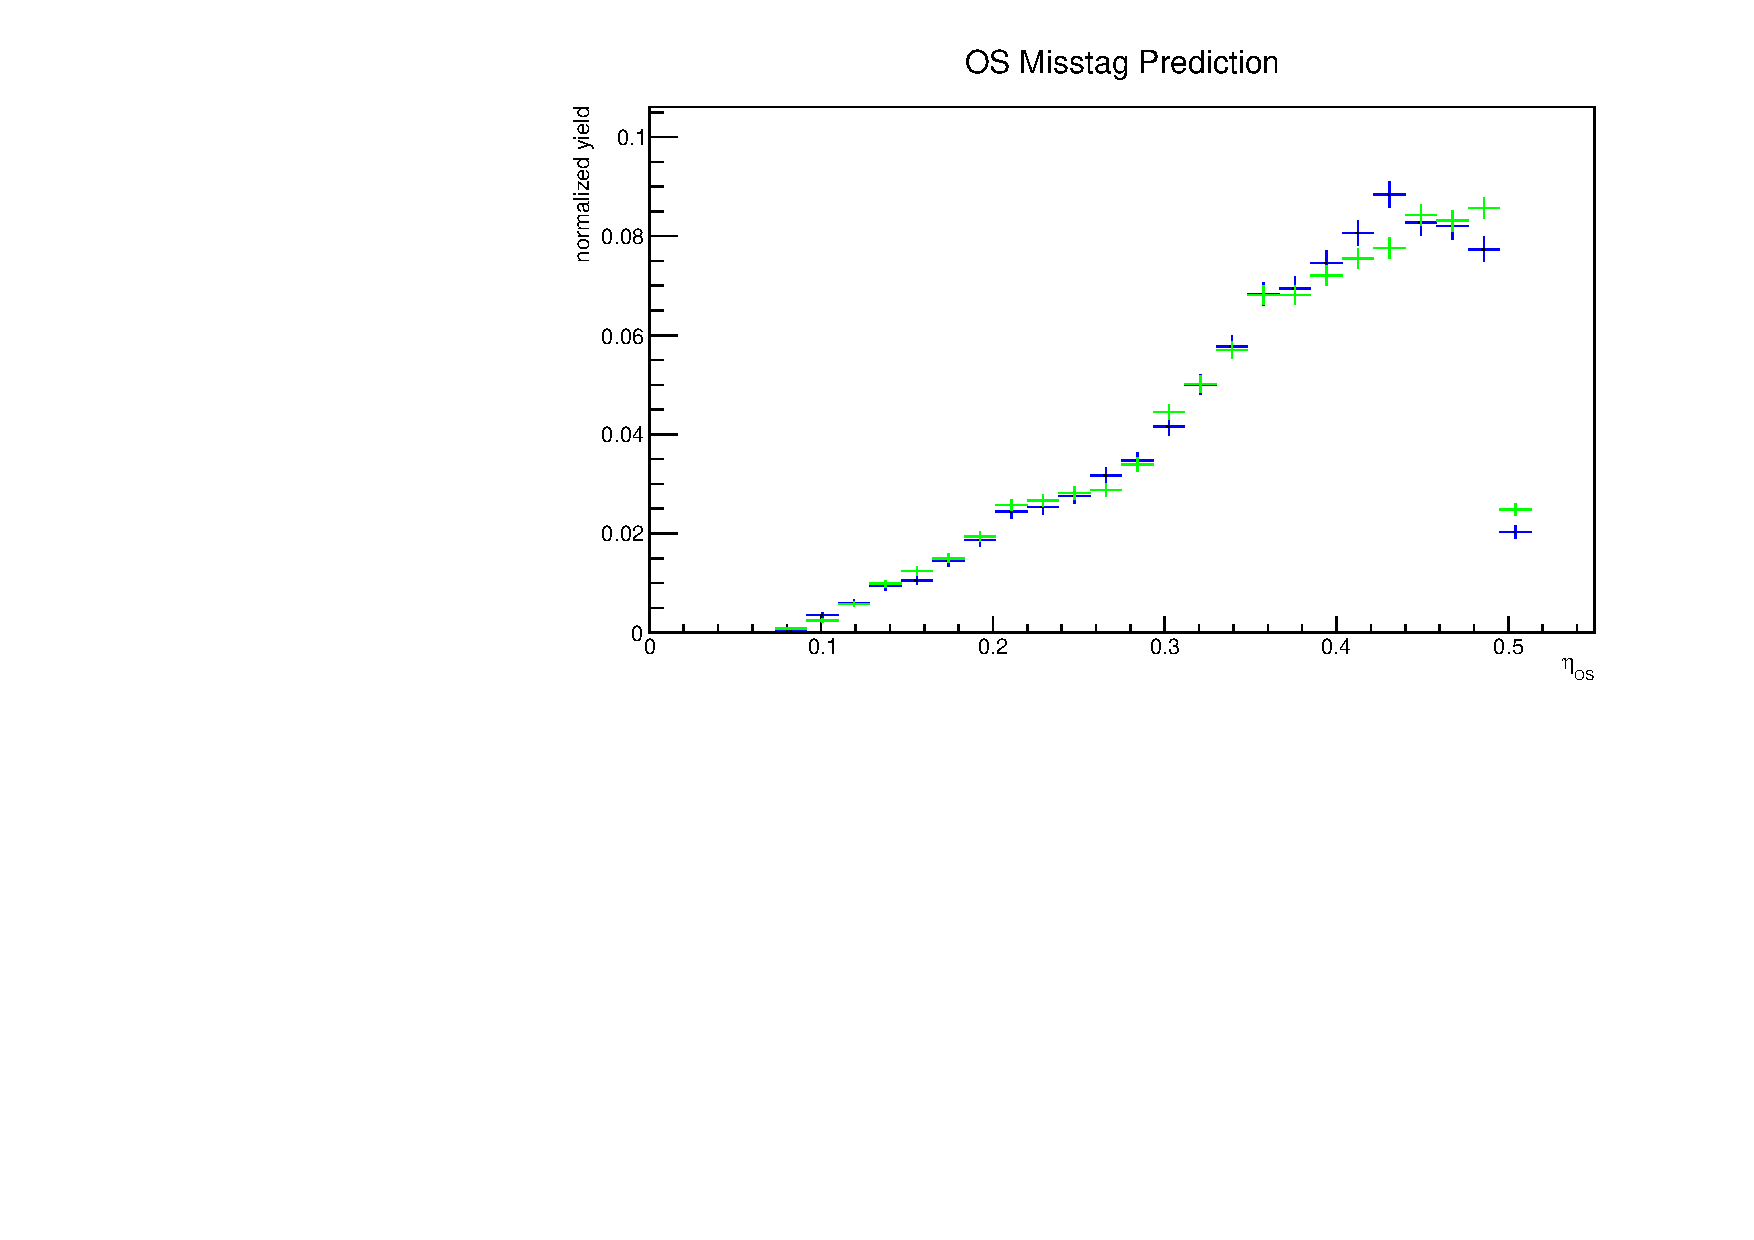
\includegraphics[height=7.cm,width=0.49\textwidth]{figs/Tagging/OS_Combination_PROB_norm_RunsComparison.pdf}
%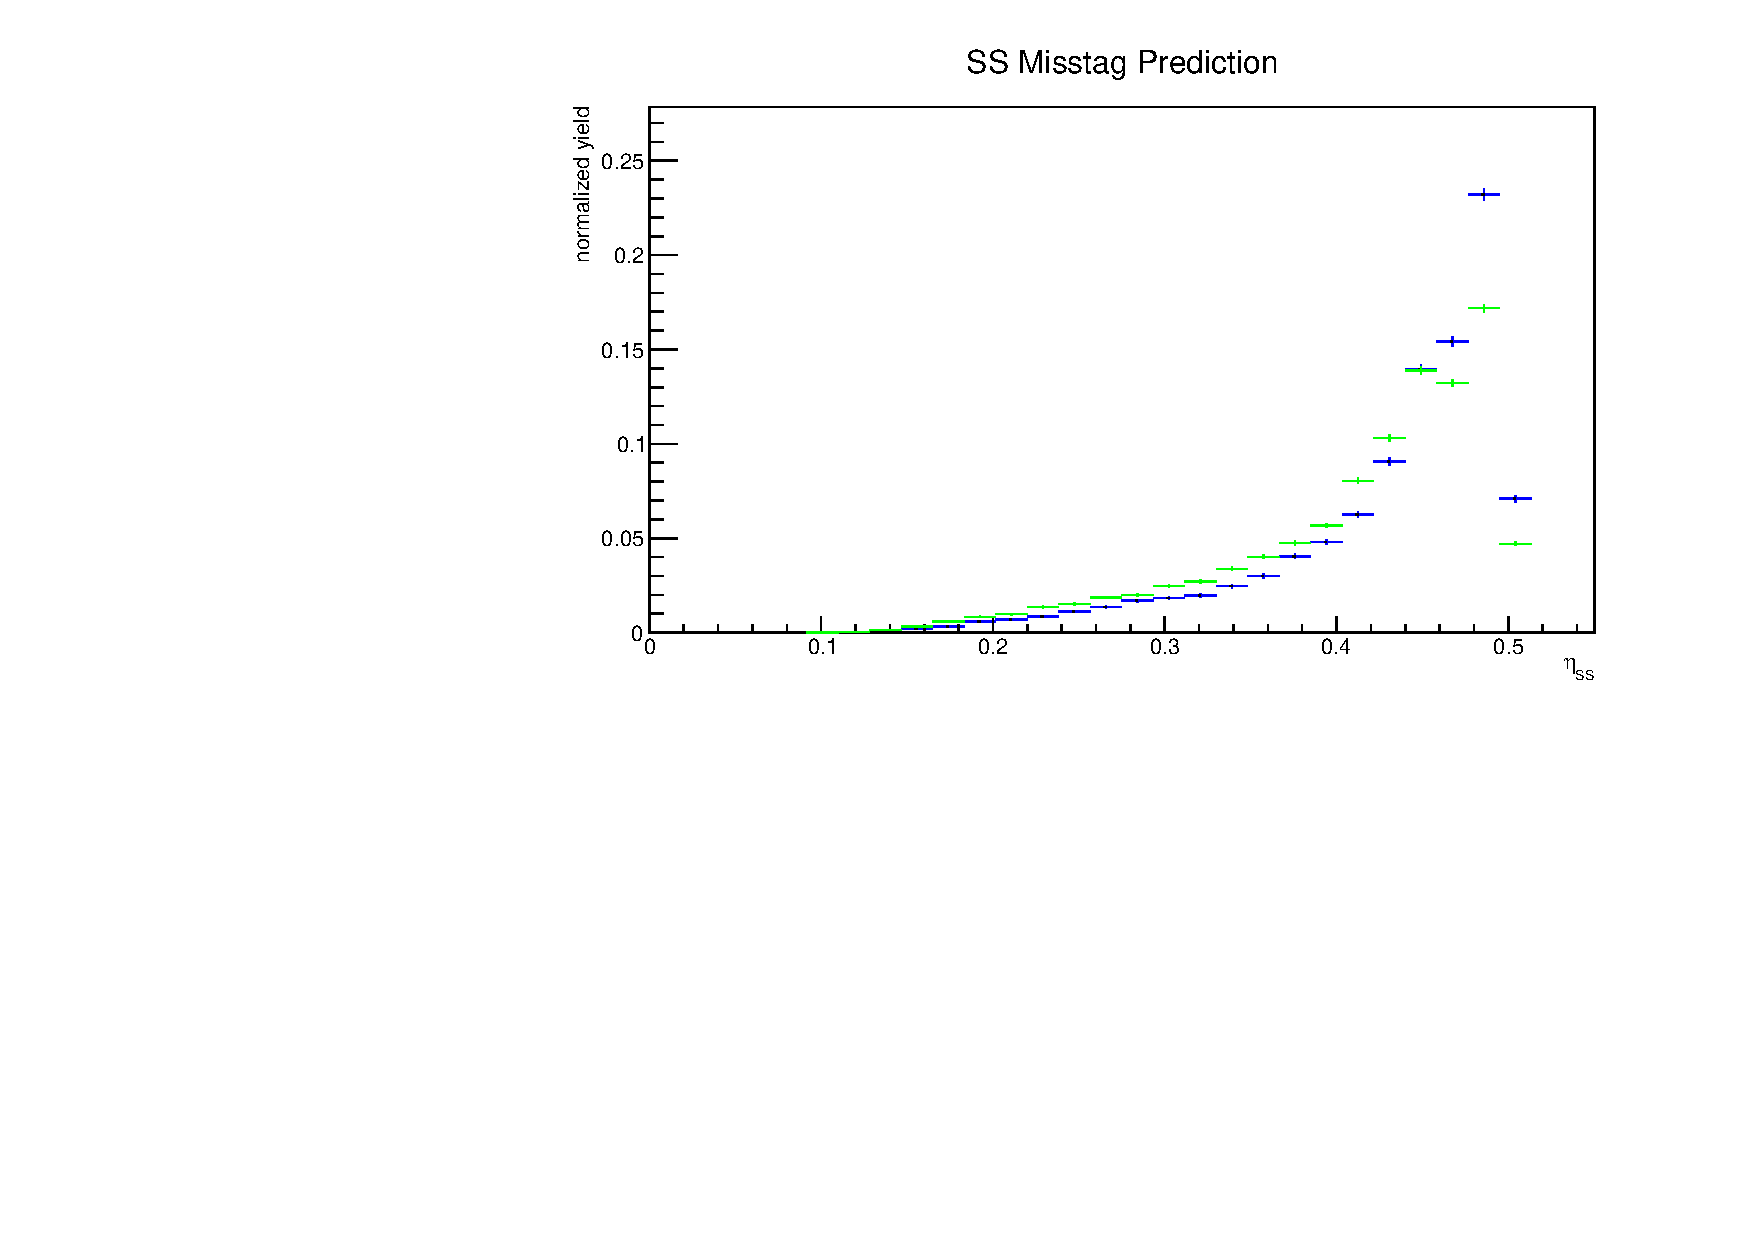
\includegraphics[height=7.cm,width=0.49\textwidth]{figs/Tagging/SS_nnetKaon_PROB_norm_RunsComparison.pdf}
%\caption{Distributions of the tagging decision from the OS combination (upper left) and the SS kaon tagger (upper right), 
%as well as the predicted mistag $\eta$ for OS (bottm left) and the SS  (bottom right), for $\Bs\to\Ds\pion\pion\pion$ candidates in the Run 1 (blue) and Run 2 (green) data samples. 
%The signal distributions are obtained using sWeights, the procedure is described in Sec. \ref{subsec: sWegihts}.}
%\label{fig:kinematics_data_comparison}
%\end{figure}

%Fig. \ref{fig:kinematics_data_comparison} shows the signal data distributions of the transverse $\Bs$ momentum $\pt$, the pseudorapidity $\eta$ of the signal candidate and the number of reconstructed tracks per event.
%Sufficient agreement is observed.

%\begin{figure}[h]
%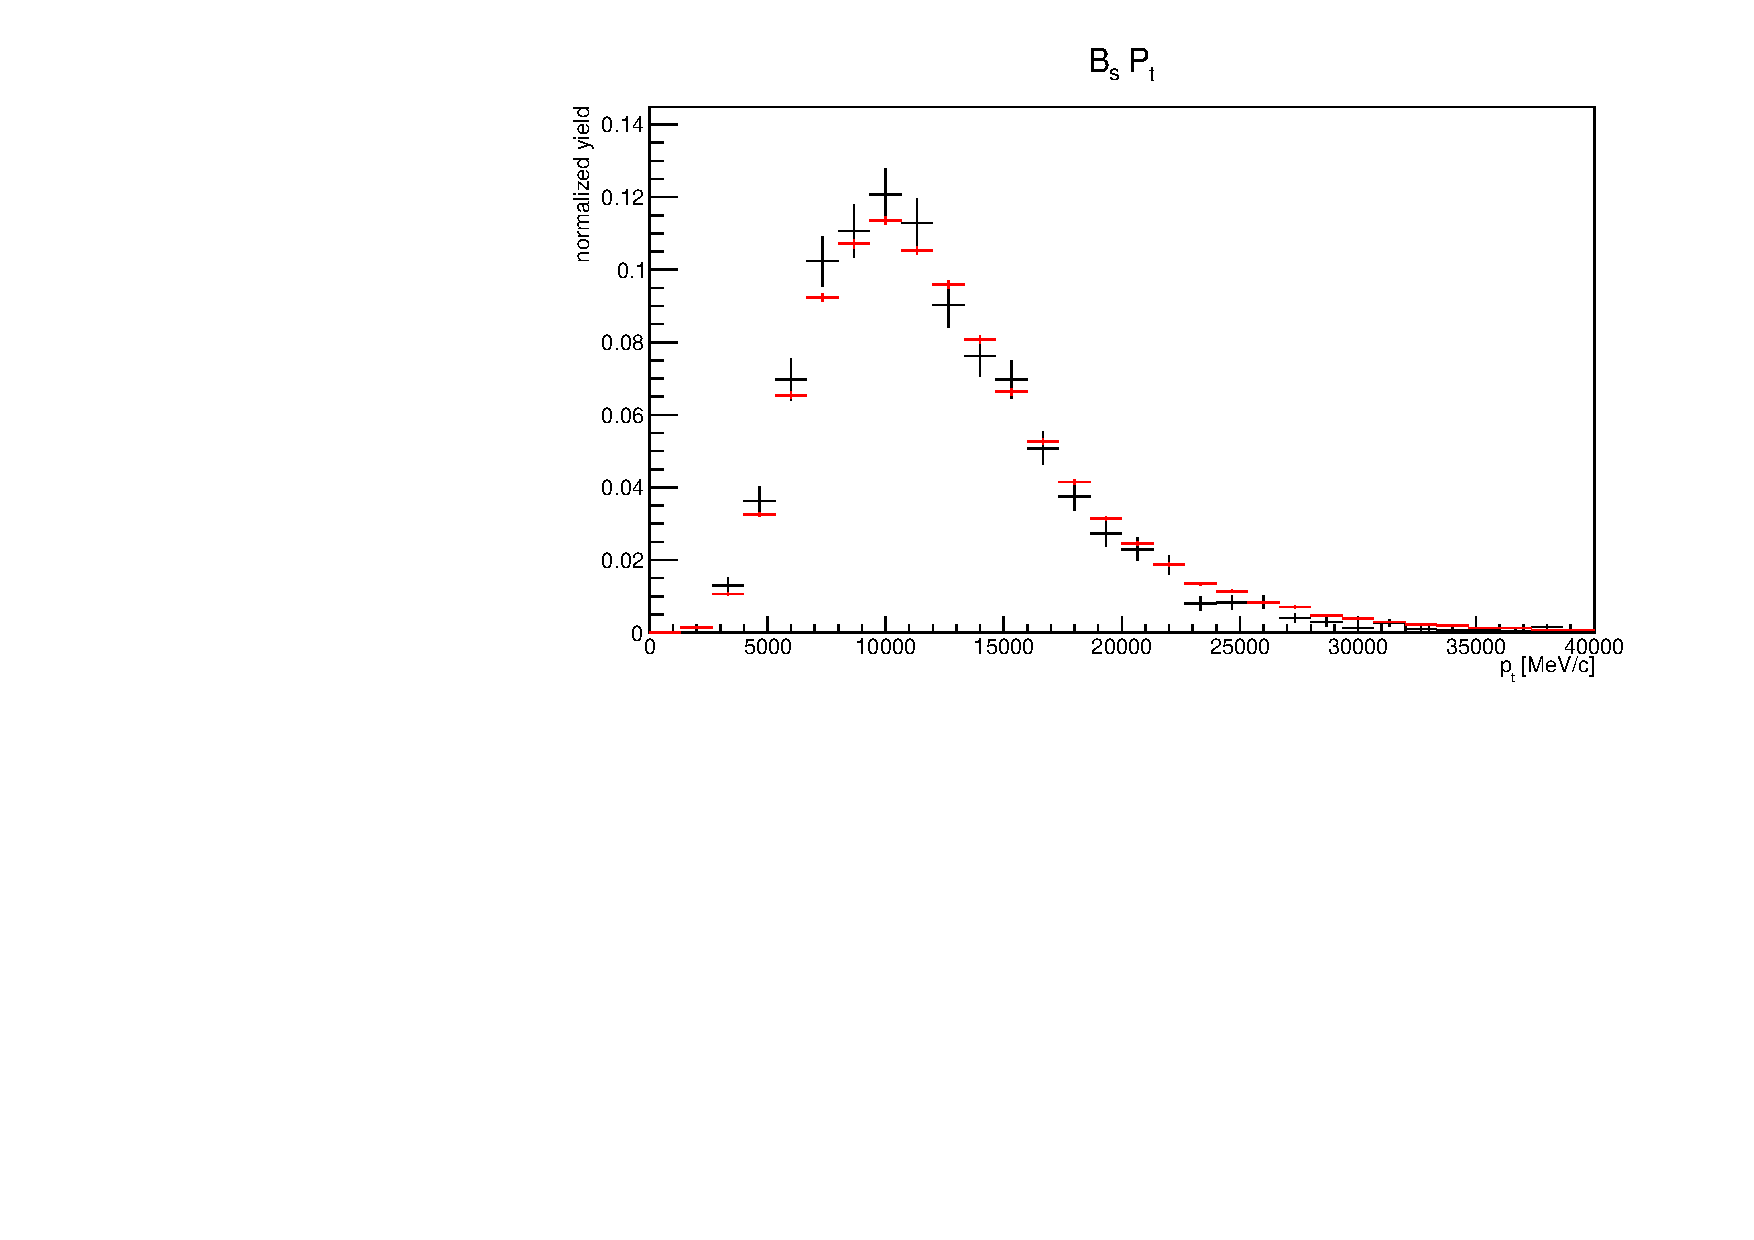
\includegraphics[height=7.cm,width=0.49\textwidth]{figs/Tagging/Bs_Pt_comparison.pdf}
%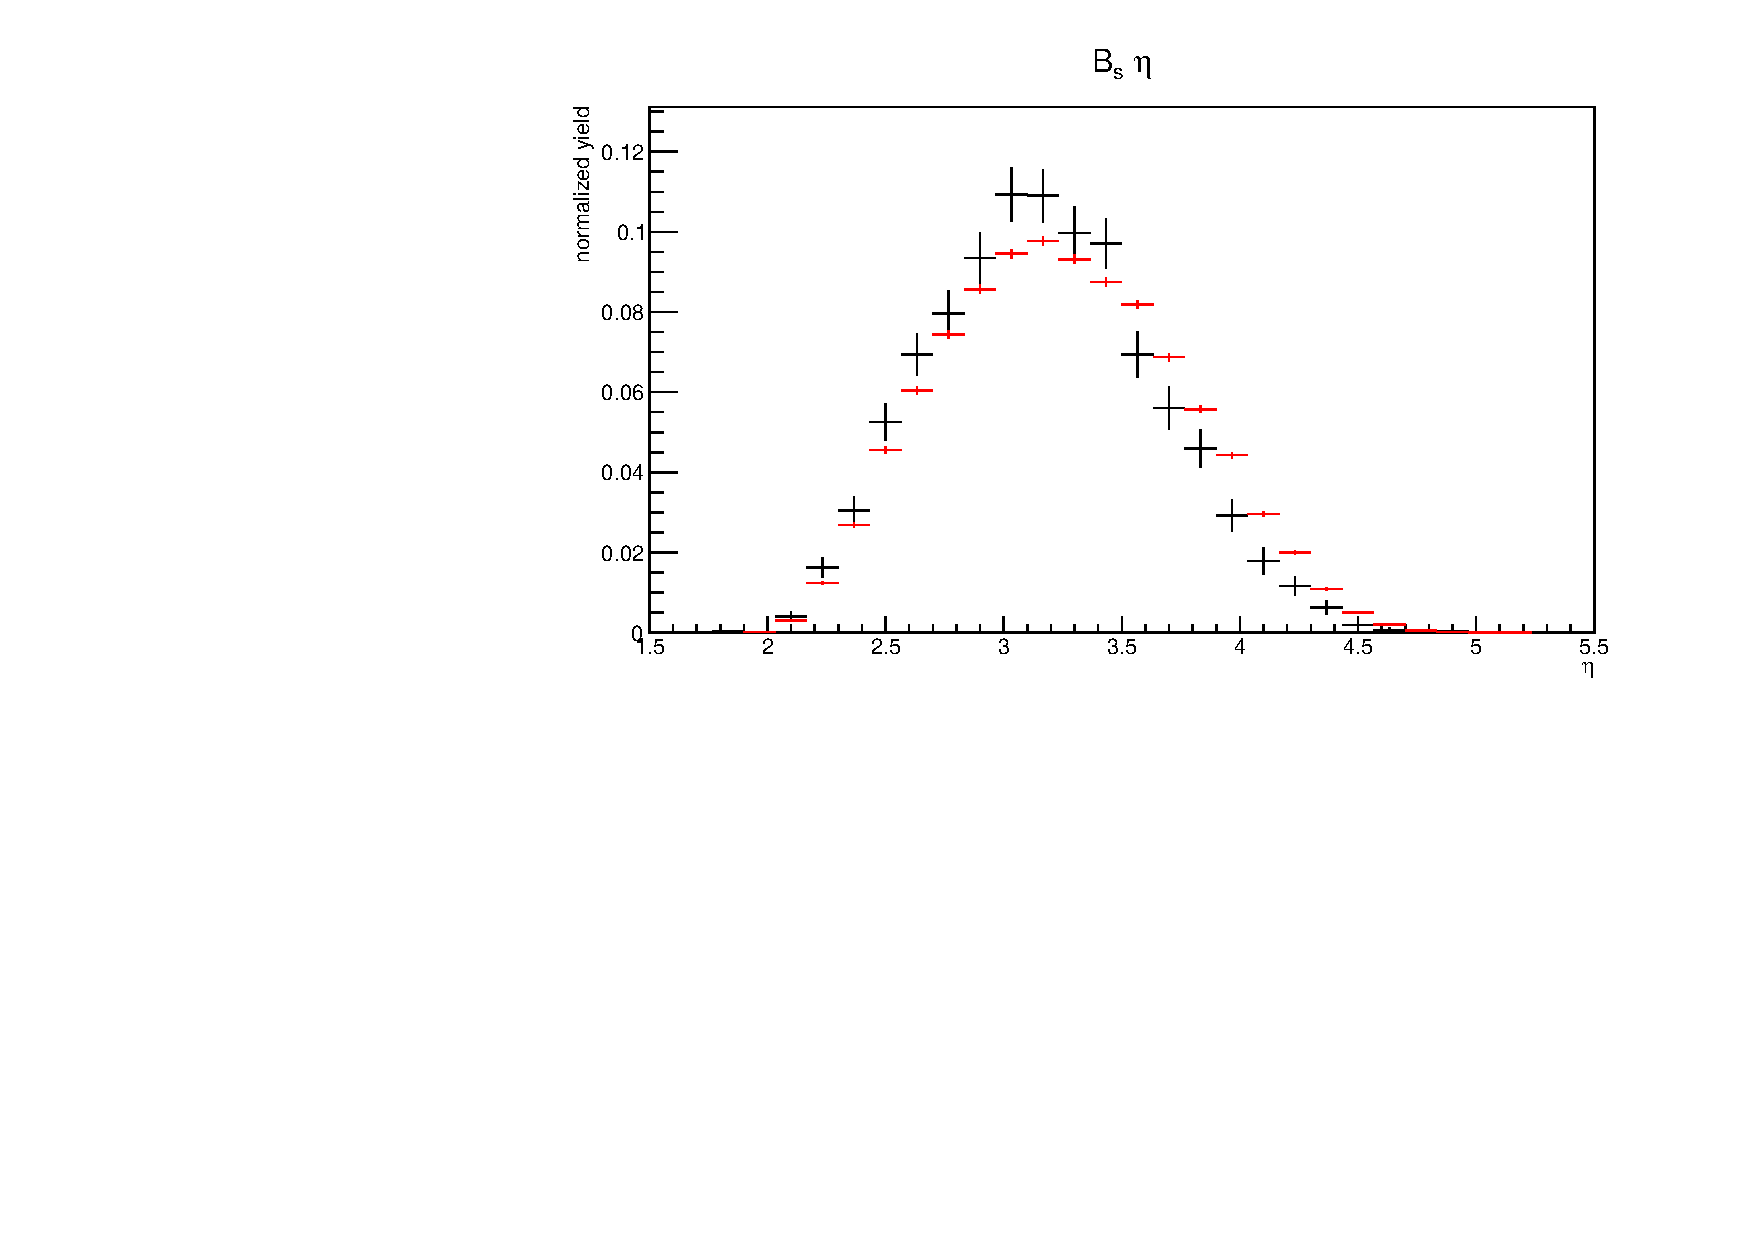
\includegraphics[height=7.cm,width=0.49\textwidth]{figs/Tagging/Bs_eta_comparison.pdf}\\
%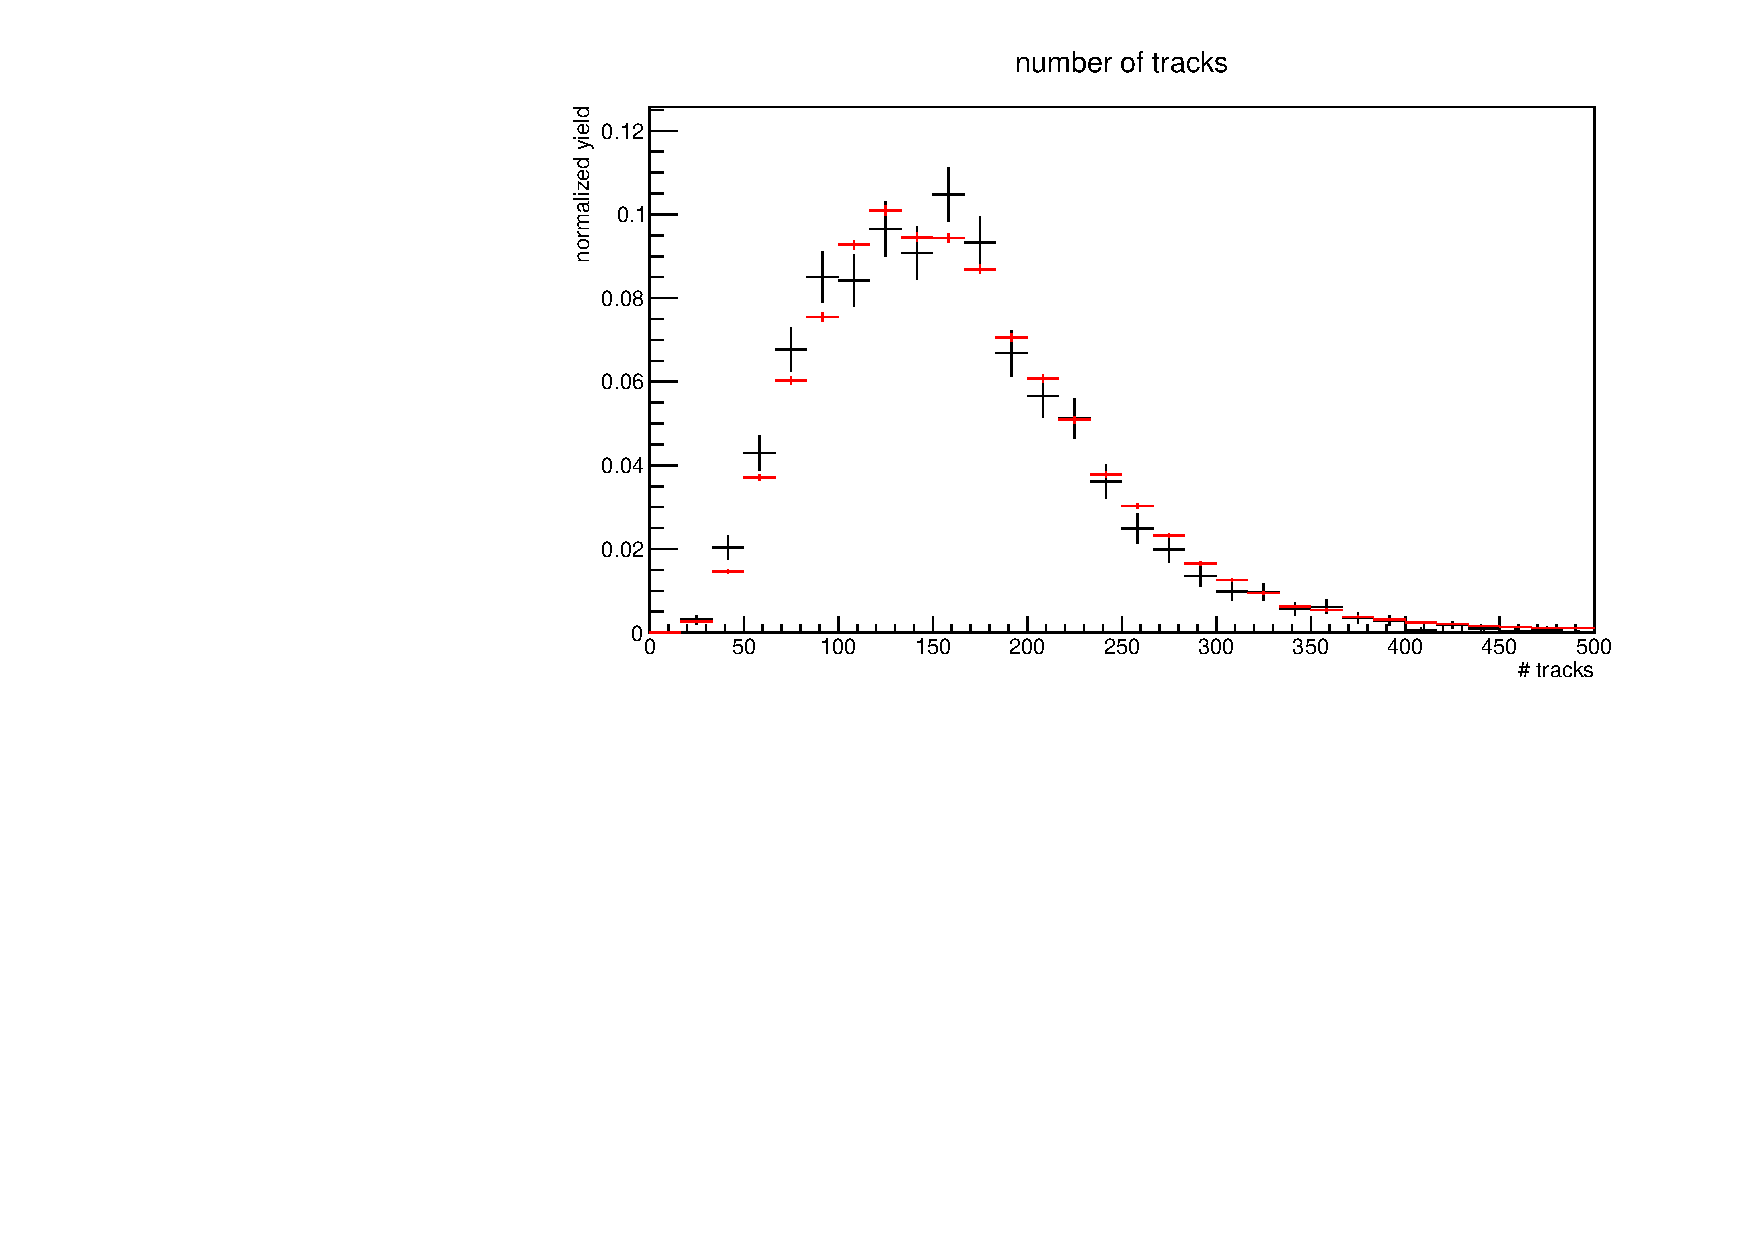
\includegraphics[height=7.cm,width=0.49\textwidth]{figs/Tagging/nTracks_comparison.pdf}
%\caption{Distributions of the transverse momentum $\pt$ (top left), 
%the pseudorapidity $\eta$ (top right) and the reconstructed number of tracks in the event (bottom left) for signal candidates in the $\Bs\to\Ds\kaon\pion\pion$ (black) and $\Bs\to\Ds\pion\pion\pion$ (red) data samples. 
%The signal distributions are obtained using sWeights, the procedure is described in Sec. \ref{subsec: sWegihts}.}
%\label{fig:kinematics_data_comparison}
%\end{figure}

%\begin{figure}[h]
%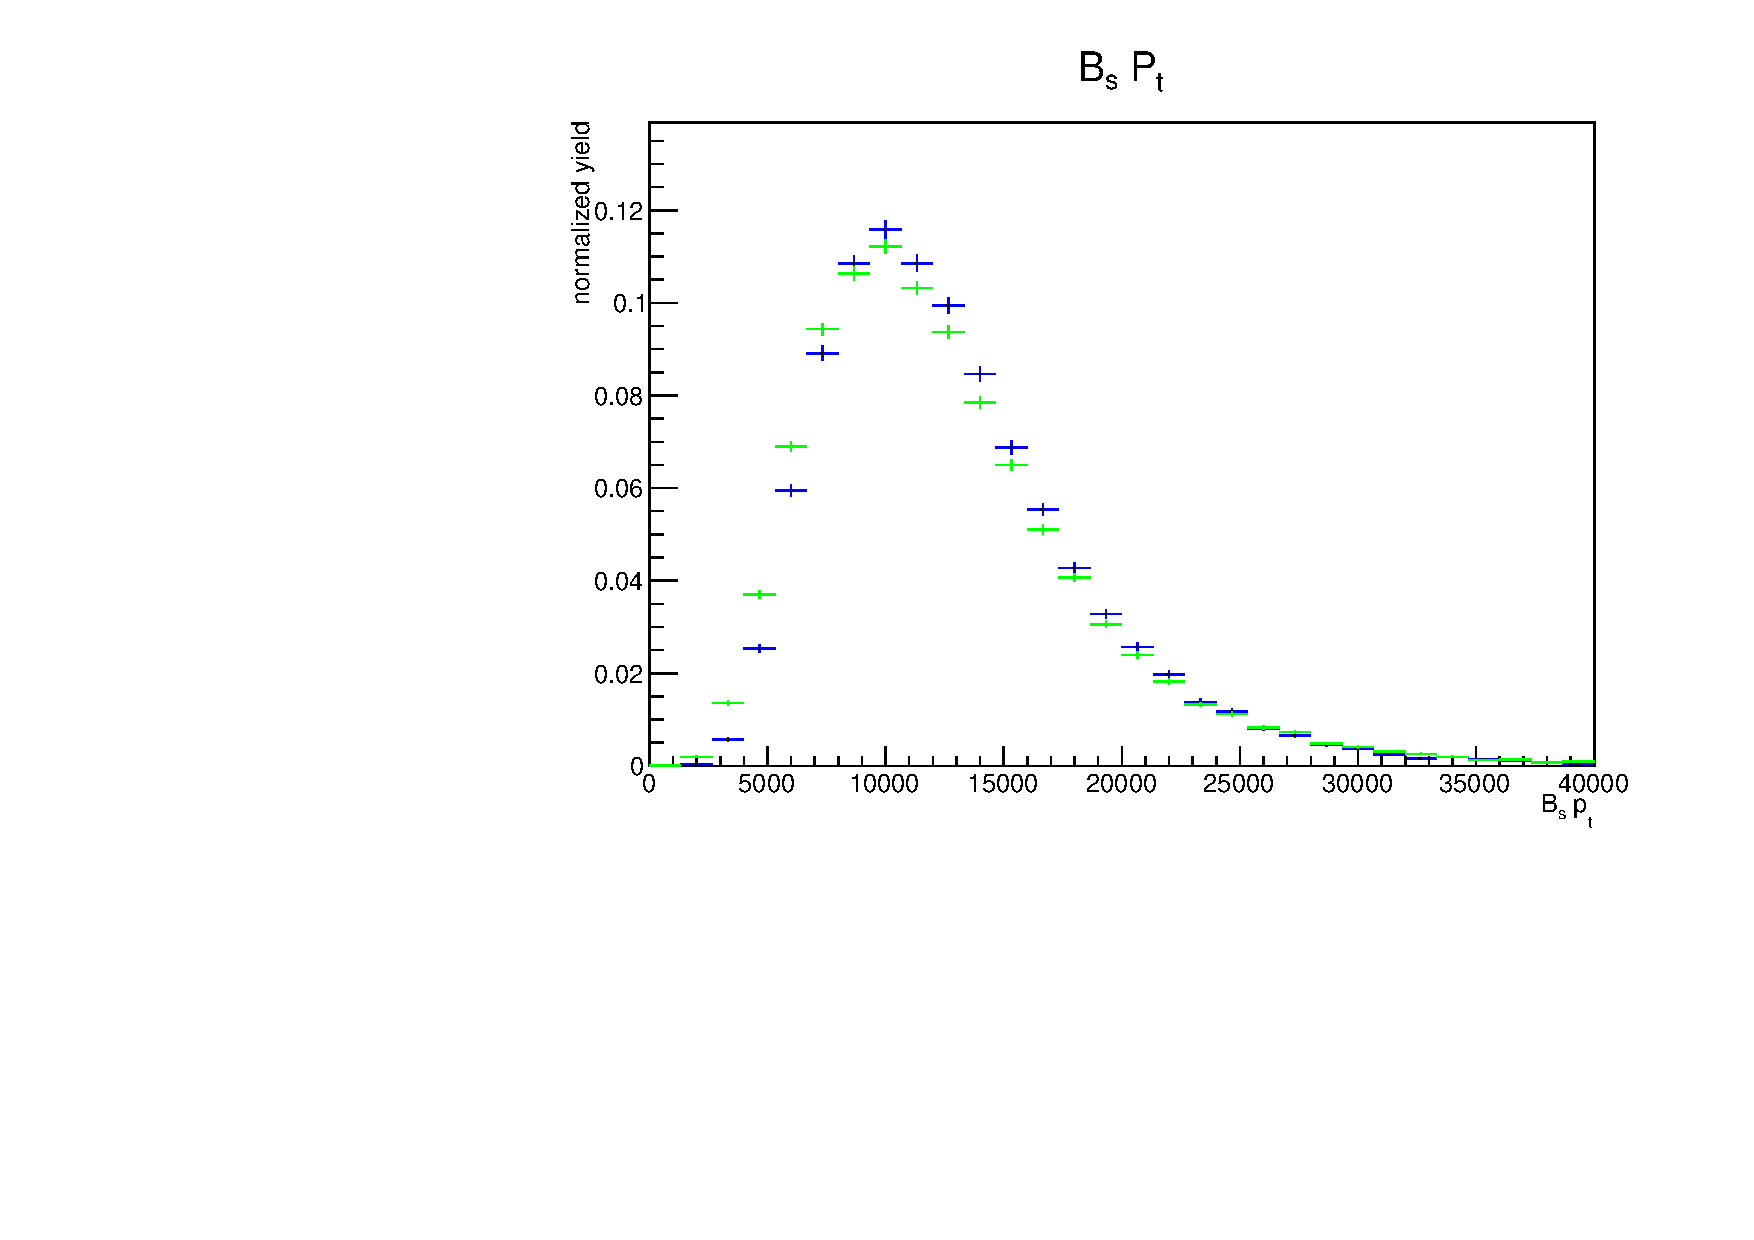
\includegraphics[height=7.cm,width=0.49\textwidth]{figs/Tagging/Bs_Pt_norm_RunsComparison.pdf}
%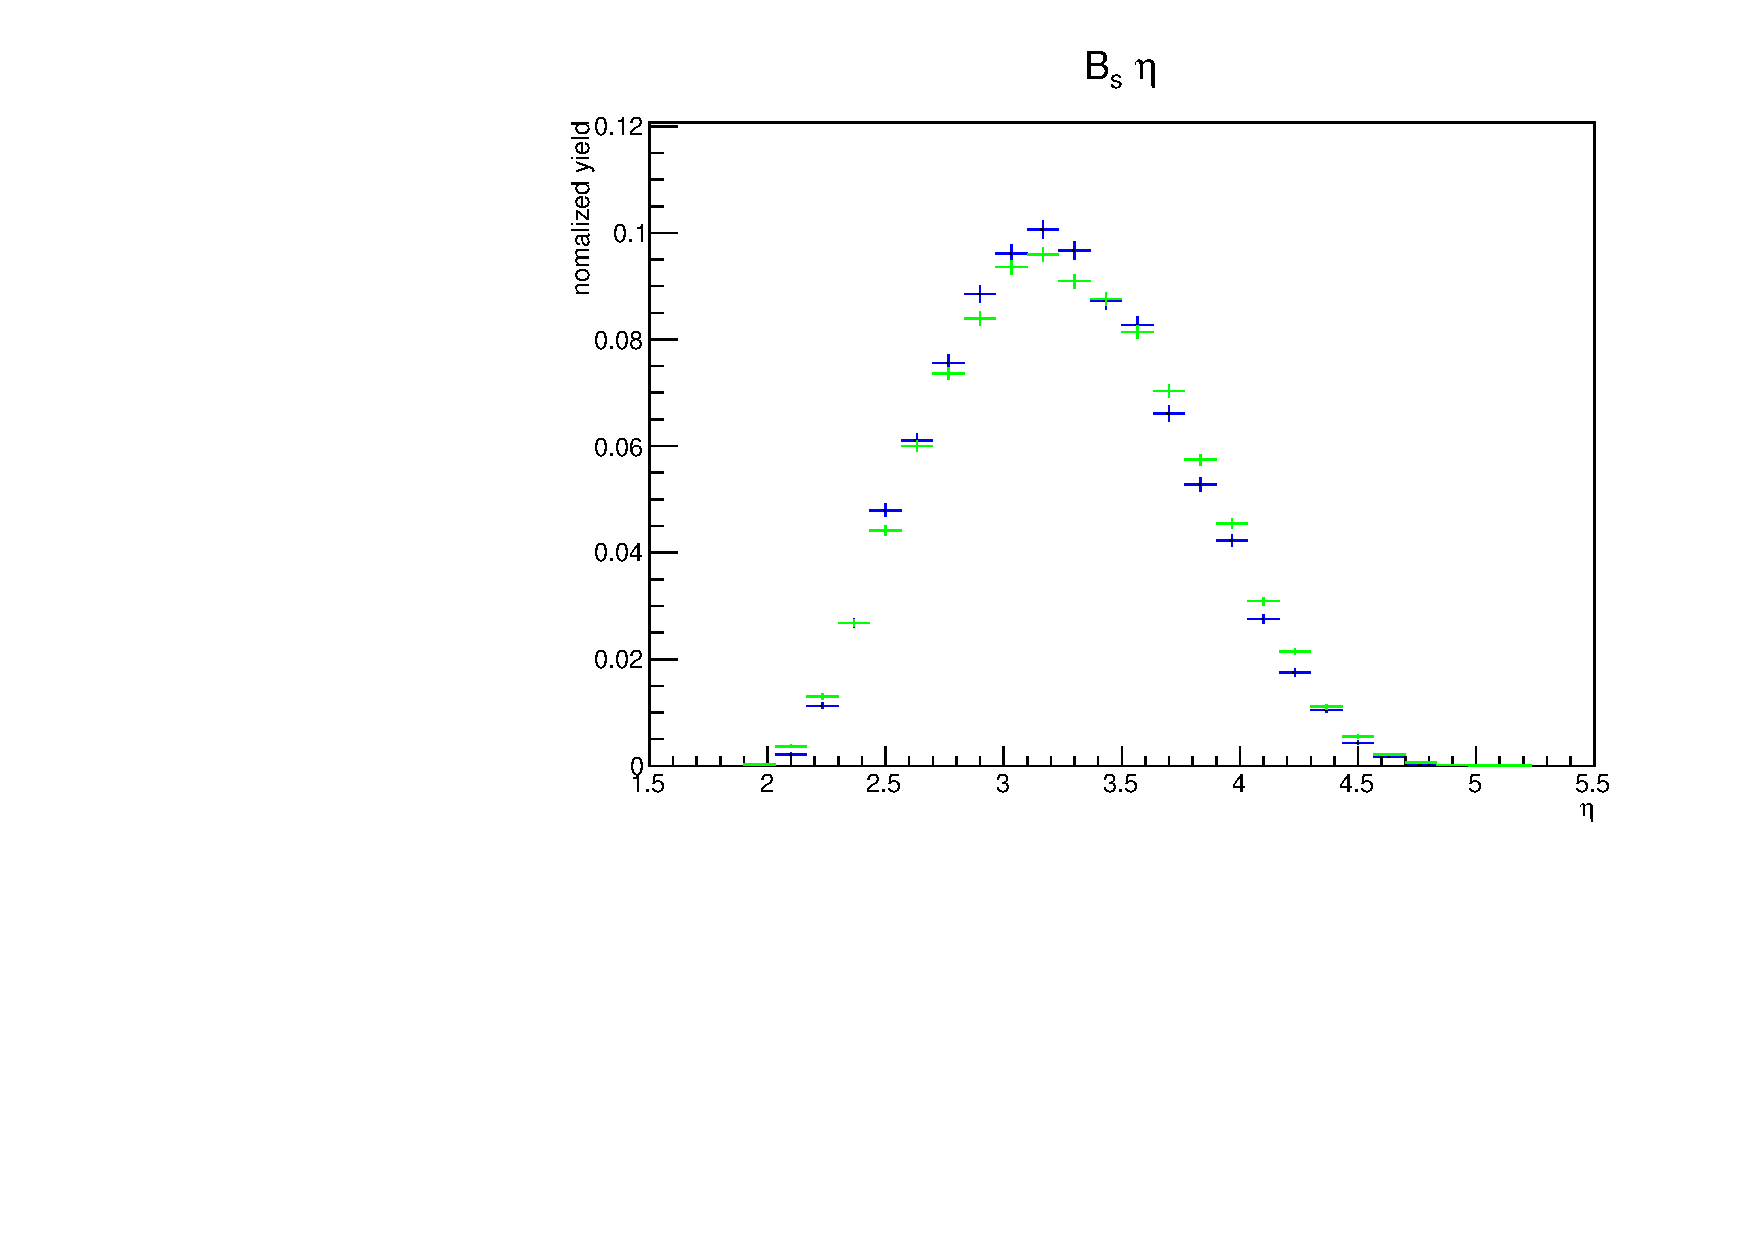
\includegraphics[height=7.cm,width=0.49\textwidth]{figs/Tagging/Bs_eta_norm_RunsComparison.pdf}\\
%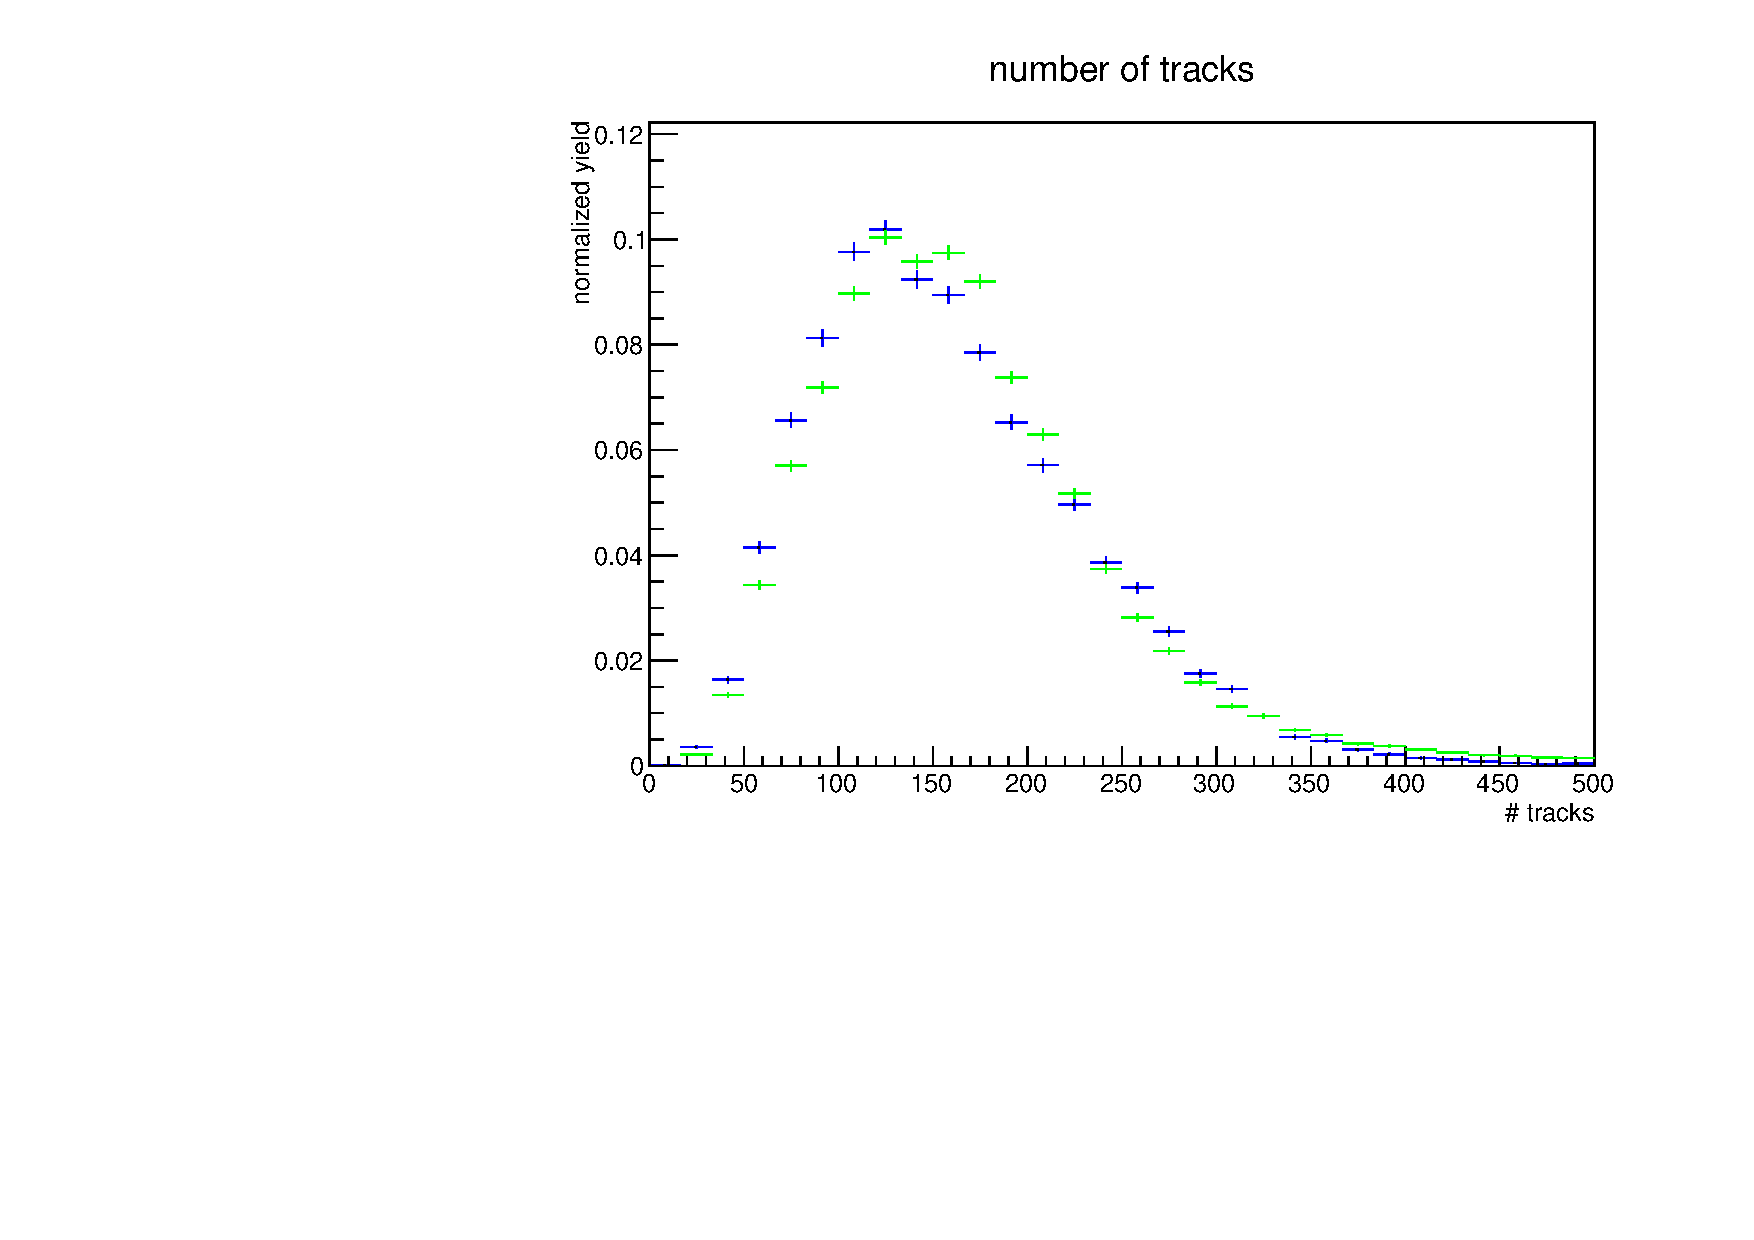
\includegraphics[height=7.cm,width=0.49\textwidth]{figs/Tagging/nTracks_norm_RunsComparison.pdf}
%\caption{Distributions of the transverse momentum $\pt$ (top left), 
%the pseudorapidity $\eta$ (top right) and the reconstructed number of tracks in the event (bottom left) for  $\Bs\to\Ds\pion\pion\pion$ candidates in the Run 1 (blue) and Run 2 (green) data samples. 
%The signal distributions are obtained using sWeights, the procedure is described in Sec. \ref{subsec: sWegihts}.}
%\label{fig:kinematics_data_comparison}
%\end{figure}

%To justify the portability of the flavour tagging calibration obtained from $\Bs\to\Ds\pion\pion\pion$ to the $\Bs\to\Ds\kaon\pion\pion$ channel, 
%besides the good agreement of the distributions shown above, the dependence of the measured mistag $\omega$ on the predicted mistag $\eta$ has to be compatible in both channels.
%This dependence is shown in Fig. \ref{fig:etavsW_mc_comparison} for simulated signal events of both channels, where good agreement is observed. 
%
%\begin{figure}[h]
%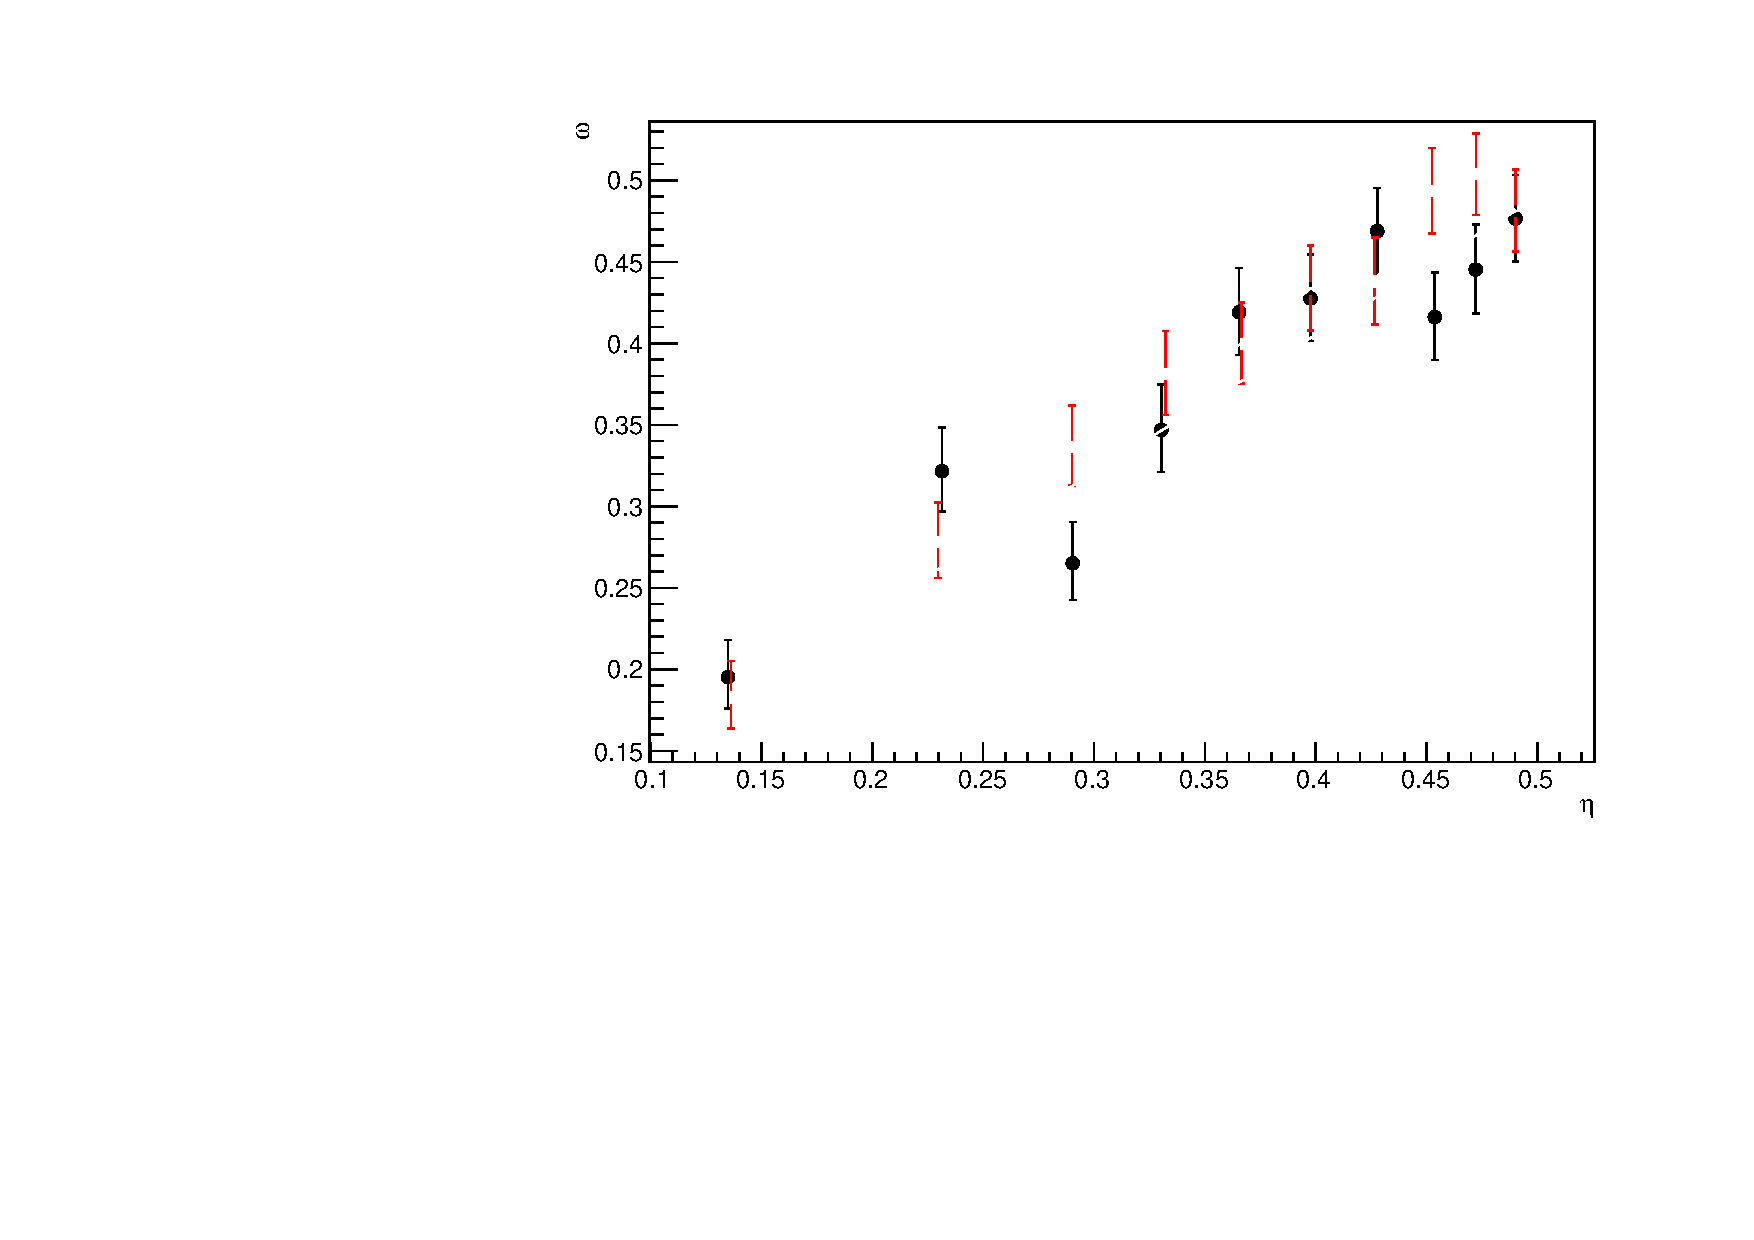
\includegraphics[height=7.cm,width=0.49\textwidth]{figs/Tagging/OS_combination_MCcomparison.pdf}
%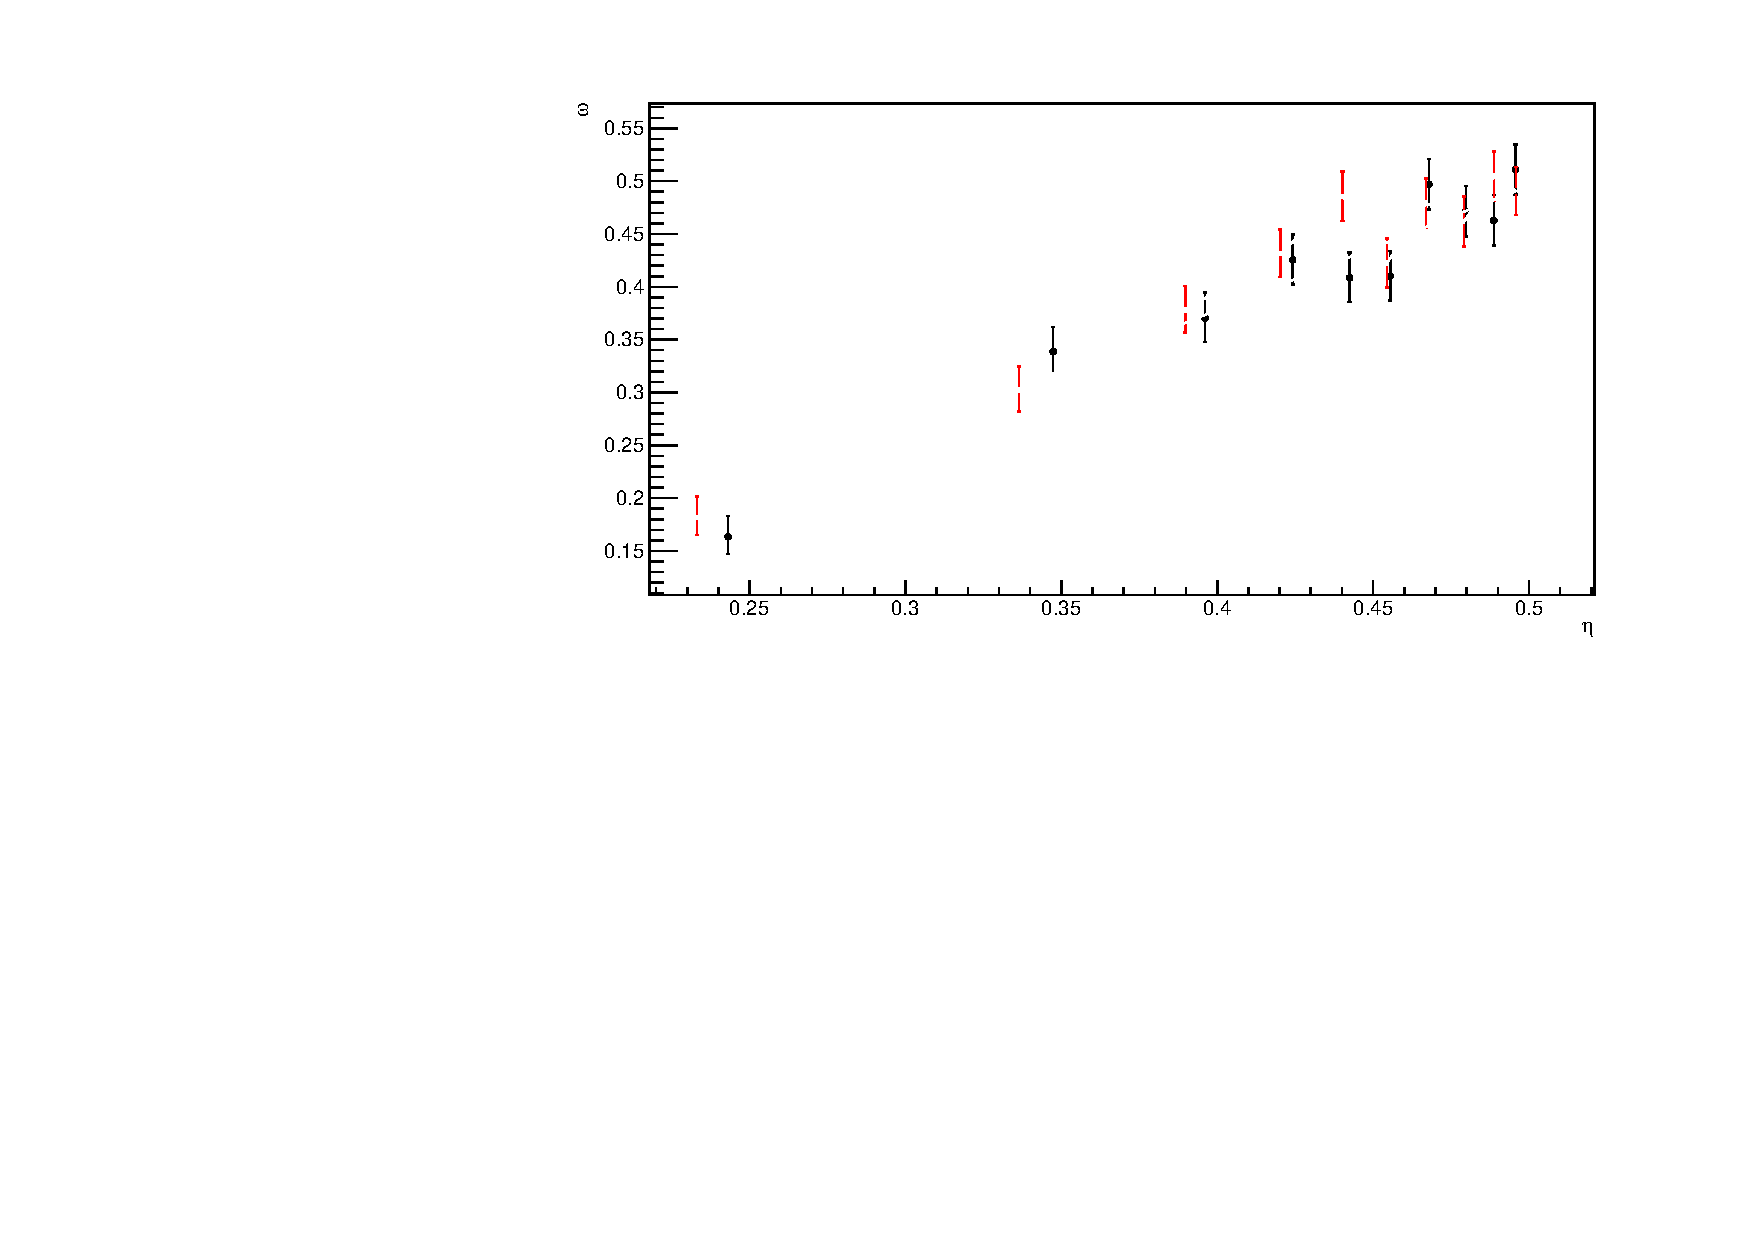
\includegraphics[height=7.cm,width=0.49\textwidth]{figs/Tagging/SS_nnetKaon_MCcomparison.pdf}
%\caption{Dependence of the observed mistag $\omega$ on the predicted mistag $\eta$ for the (left) OS combination and the (right) SS kaon tagger, 
%found in the simulated $\Bs\to\Ds\kaon\pion\pion$ (black) and $\Bs\to\Ds\pion\pion\pion$ (red) signal samples.}
%\label{fig:etavsW_mc_comparison}
%\end{figure}
%

%\subsection{Combination of OS and SS taggers}
%\label{subsec: TaggingCombination}
%
%In the time- and ampitude-dependent fit to $\Bs\to\Ds\kaon\pion\pion$ data, the obtained tagging responses of the OS and SS tagger will be combined after the calibration described in the previous sections is applied.
%Events that aquire a mistag probability greater than 0.5 after the calibration will have their tagging decision flipped. For events where only one of the two taggers fired, the combination of the tagging decision is trivial.
%In those events where both taggers made a decision, we use the standard combination of taggers \cite{LHCb-PAPER-2011-027} provided by the flavour tagging group. 
%In the nominal fit, the calibrated mistags $\omega$ are combined event by event for the OS and SS tager, thus adding one observable to the fit procedure. 
%This ensures that the uncertainties of the OS and SS tagging calibration parameters are propagated properly to the combined tagging response for each event. \newline
%The taggging performance for the combined tagger in the categories SS tagged only, 
%OS tagged only and SS+OS tagged, are shown in (Run 1) Tab. \ref{table:tagging_Run1} and (Run 2) Tab. \ref{table:tagging_Run1}.
%%The distribution of the observed mistag $\omega$ as a function of the combined mistag probability $\eta$ for $\Bs\to\Ds\pion\pion\pion$ decays is shown in Fig. \ref{fig:TaggingCombinationCalibration}.
%

\begin{table}[h]
\centering
\caption{The flavour tagging performances for only OS tagged, only SS tagged and both OS and SS tagged events for Run-I data.}
\begin{tabular}{c c c c}
\hline
\hline
$ B_s \to D_s \pi \pi \pi$ & $\epsilon_{tag} [\%]$ & $\langle \omega \rangle [\%] $ & $\epsilon_{eff} [\%]$ \\
\hline
Only OS & 14.74 $\pm$ 0.11 & 39.09 $\pm$ 0.80 & 1.25 $\pm$ 0.16\\
Only SS & 35.38 $\pm$ 0.18 & 44.26 $\pm$ 0.62 & 1.05 $\pm$ 0.18\\
Both OS-SS & 33.04 $\pm$ 0.30 & 37.33 $\pm$ 0.73 & 3.41 $\pm$ 0.33\\
\hline
Combined & 83.16 $\pm$ 0.37 & 40.59 $\pm$ 0.70 & 5.71 $\pm$ 0.40\\
\hline
\hline
\end{tabular}

\label{tab:tagPerfRun1}

\caption{The flavour tagging performances for only OS tagged, only SS tagged and both OS and SS tagged events for Run-II data.}
\begin{tabular}{c c c c}
\hline
\hline
$ B_s \to D_s K \pi \pi$ & $\epsilon_{tag} [\%]$ & $\langle \omega \rangle [\%] $ & $\epsilon_{eff} [\%]$ \\
\hline
Only OS & 12.99 $\pm$ 0.06 & 37.06 $\pm$ 0.51 & 1.28 $\pm$ 0.08\\
Only SS & 39.89 $\pm$ 0.10 & 42.92 $\pm$ 0.35 & 1.63 $\pm$ 0.11\\
Both OS-SS & 28.64 $\pm$ 0.14 & 35.50 $\pm$ 0.40 & 3.59 $\pm$ 0.16\\
\hline
Combined & 81.53 $\pm$ 0.18 & 39.38 $\pm$ 0.40 & 6.50 $\pm$ 0.21\\
\hline
\hline
\end{tabular}

\label{tab:tagPerfRun2}
\end{table}


